\documentclass[10pt, aspectratio=169]{beamer}

% Configuration {{{
\usepackage[utf8]{inputenc}
\usepackage[T2A]{fontenc} % T1 for English
\usepackage[english, russian]{babel}

\usepackage{mathtools}
\usepackage{graphicx}
\usepackage{tikz}
\usepackage[multidot]{grffile}
\usepackage[labelsep=period]{caption}
\usepackage{multirow}

\setbeamertemplate{caption}[numbered]
\setbeamertemplate{navigation symbols}{}
\usefonttheme[onlymath]{serif}
\usepackage{DejaVuSansCondensed} % helvet for English
\usetheme{Madrid}

\linespread{1.2}
% }}}

% Definitions {{{
\def\todo#1{\colorbox{orange}{TODO: #1}}

\def\Lb{{\Lambda_b^0}}
\def\Lc{{\Lambda_c^+}}
\def\Lcstar{{\Lambda_c^{*+}}{}}
\def\Lca{{\Lambda_c(2765)^+}}
\def\Lcb{{\Lambda_c(2940)^+}}
\def\LcII{{\Lambda_c(2625)^+}}
\def\LcIII{{\Lambda_c(2880)^+}}
\def\LcIIIother{{\Lambda_c(2765)^+}}
\def\ScI{{\Sigma_c(2455)}}
\def\ScIpp{{\Sigma_c(2455)^{++}}{}}
\def\ScIp{{\Sigma_c(2455)^{+}}{}}
\def\ScIz{{\Sigma_c(2455)^{0}}{}}
\def\ScII{{\Sigma_c(2520)}}
\def\ScIIpp{{\Sigma_c(2520)^{++}}{}}
\def\ScIIp{{\Sigma_c(2520)^{+}}{}}
\def\ScIIz{{\Sigma_c(2520)^{0}}{}}
\def\ScIII{{\Sigma_c(2800)}}
\def\ScIIIpp{{\Sigma_c(2800)^{++}}{}}
\def\ScIIIp{{\Sigma_c(2800)^{+}}{}}
\def\ScIIIz{{\Sigma_c(2800)^{0}}{}}
\def\Sc{{\Sigma_c}}
\def\Scpp{{\Sigma_c^{++}}{}}
\def\Scp{{\Sigma_c^{+}}{}}
\def\Scz{{\Sigma_c^{0}}{}}
\def\Scstar{{\Sigma_c^*}}
\def\Scstarpp{{\Sigma_c^{*++}}{}}
\def\Scstarp{{\Sigma_c^{*+}}{}}
\def\Scstarz{{\Sigma_c^{*0}}{}}
\def\Scoptstar{{\Sigma_c^{(*)}}{}}
\def\Scoptstarpp{{\Sigma_c^{(*)++}}{}}
\def\Scoptstarp{{\Sigma_c^{(*)+}}{}}
\def\Scoptstarz{{\Sigma_c^{(*)0}}{}}
\def\pip{{\pi^+}}
\def\pim{{\pi^-}}
\def\piz{{\pi^0}}
\def\rhop{\rho^+}
\def\rhom{\rho^-}
\def\Kp{{K^+}}
\def\Km{{K^-}}
\def\p{{p}}
\def\Dz{{D^0}}
\def\Dzbar{{\bar{D}^0}}
\def\Dp{{D^+}}
\def\Dsubsm{{\bar{D}_s^0}}
\def\Dsubsp{{D_s^+}}
\def\Dstarp{{D^{*+}}{}}
\def\Dstarz{{D^{*0}}{}}
\def\Dstarzbar{{\bar{D}^{*0}}{}}
\def\Bz{{B^0}}
\def\Bsz{{B_s^0}}
\def\gevcc{{GeV$/c^2$}}
%}}}

% Title and other {{{
\title[Measurements of $b$-hadron BRs at the LHCb]{
  Measurements of branching ratios of $b$-hadrons
  \\ at the LHCb detector
}
\author[Kerim Guseynov]{
  Kerim Guseynov
  \vskip 1ex
  \scriptsize
  Based on analyses by the LHCb Collaboration: \\
  First observations of $B^0_s\to D^+D^-$, $D^+_sD^-$ and $D^0\bar{D}^0$ decays,
  Phys. Rev. D 87, 092007 (2013), \\
  Observation of the $B^0 \to \bar{D}^{*0}K^+\pi^-$ and $B_s^0 \to \bar{D}^{*0}K^-\pi^+$ decays,
  Phys. Rev. D 105, 072005 (2022), \\
  Observation of $\Lb\to\Dp p\pim\pim$ and $\Lb\to\Dstarp p\pim\pim$ decays,
  JHEP 03 153 (2022).
  %\todo{What else?}
}
\institute[MSU]{
  Faculty of Physics \\ Moscow State University
}
\date{March 27, 2023}
%}}}

\begin{document}

\frame[plain]{\titlepage}

\begin{frame}[label=intro]%{{{
  \frametitle{Introduction}

  Measurements of nonleptonic $b$-hadron decays allow one to

  \begin{itemize}
    \item Probe the CKM Matrix parameters:
      determine transition rates between quarks,
    \item Study final state interactions,
    \item Test theoretical calculations:
      perturbative, non-perturbative, phenomenological,

    \item Improve our knowledge of hadron spectroscopy.
  \end{itemize}

  \vfill

  The $\gamma$ of the CKM matrix is of especially
  high priority in modern particle physics.
  Its measurement can be improved by investigating both
  larger data samples and new decays.

\end{frame}%}}}

\begin{frame}[label=lhcb]%{{{
  \frametitle{The LHCb detector at the LHC}
  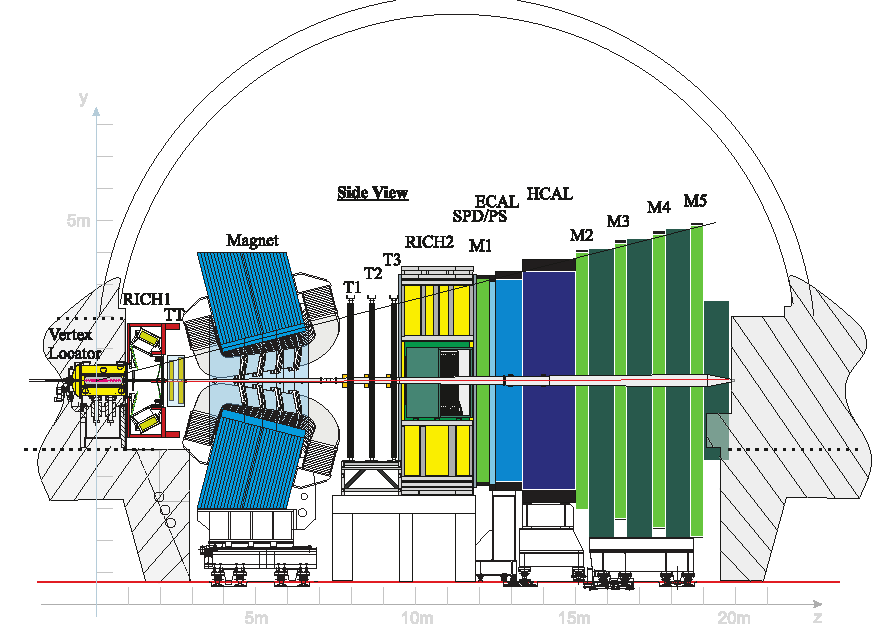
\includegraphics[width=.59\linewidth]{figures/conf/lhcb-detector}
  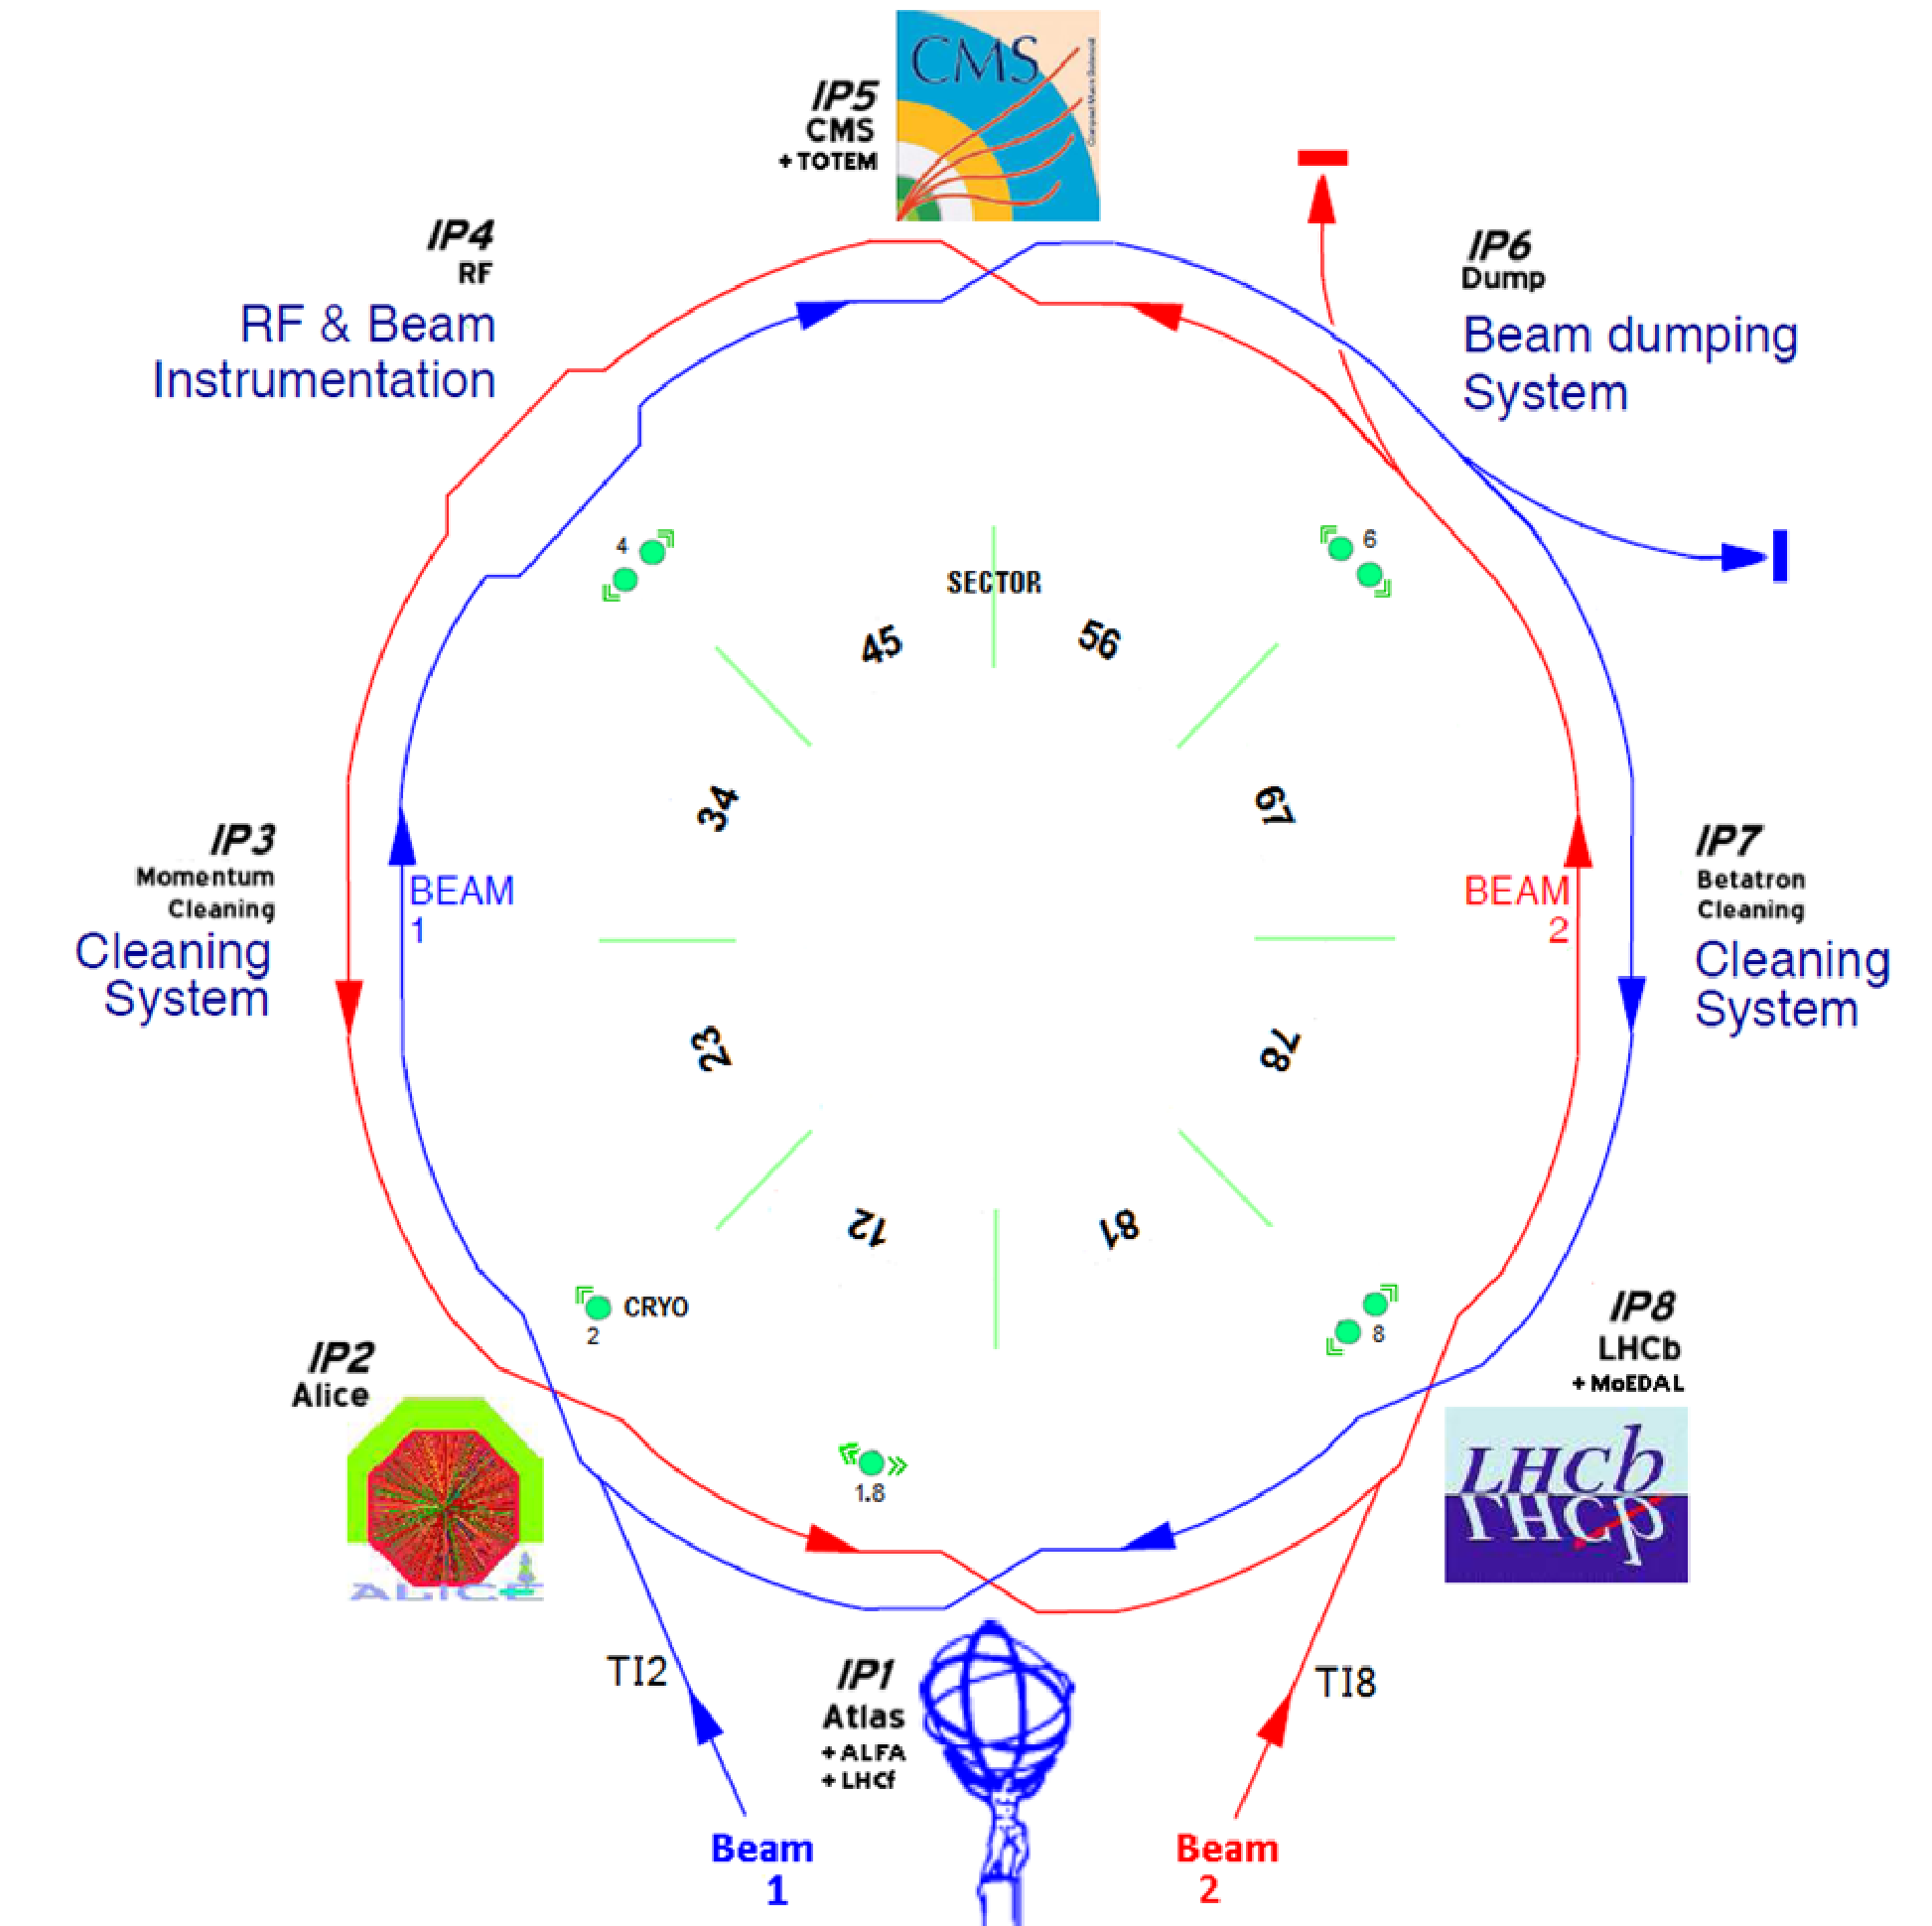
\includegraphics[width=.39\linewidth]{figures/conf/lhc-ring}

  %\hfill \todo{cite [JINST 3 S08005]? cite pic sources?} \hfill \null

  % The LHCb detector is at the forefront of modern particle physics.
  % It is located at the Large Hadron Collider in Europe in Geneva
  % and it is one of the four major experiments at the LHC.
  % The detector itself is tailored specifically for measurements
  % of bottom hadron decays and has the following main components:
  % VELO, Tracking system, Cherenkov detectors, calorimeters,
  % muon stations.
\end{frame}%}}}

\begin{frame}[label=decays]%{{{
  \frametitle{The decays under the study}

  \centering

  \begin{tabular}{cc}
    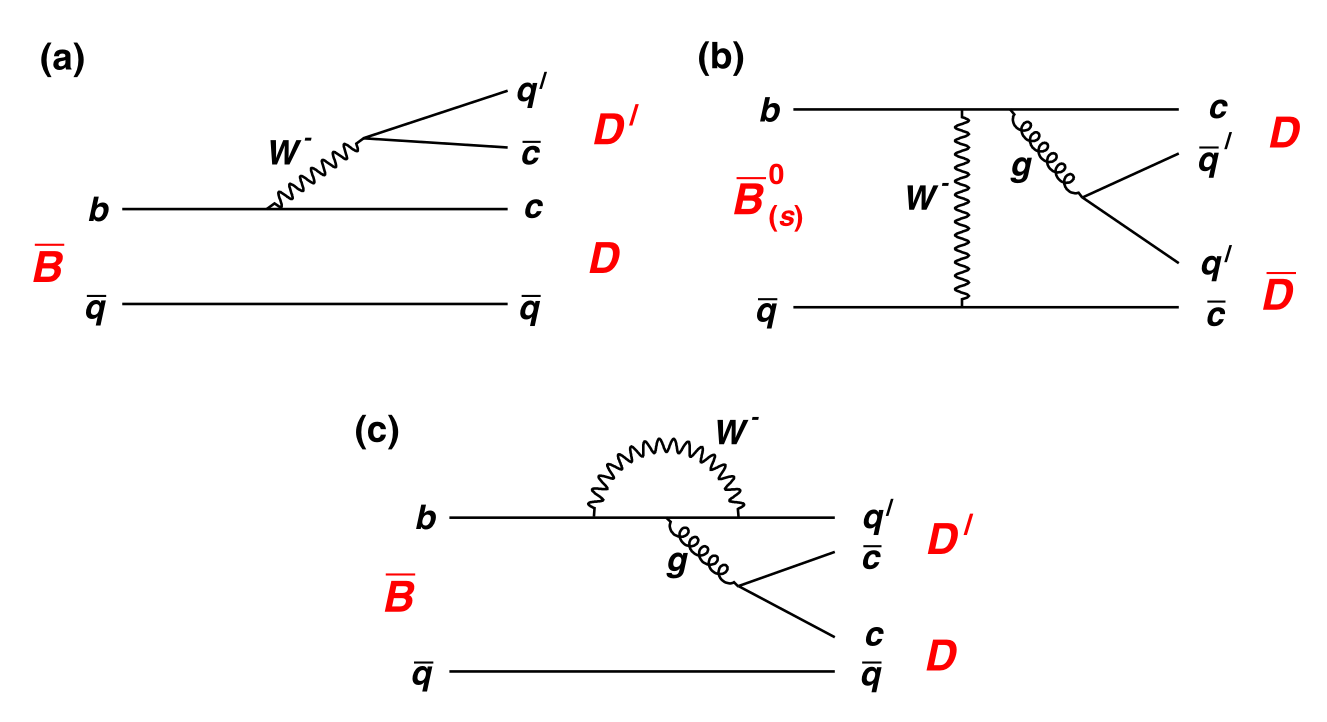
\includegraphics[width=.4\linewidth]{figures/conf/B2DD-fig001} &
    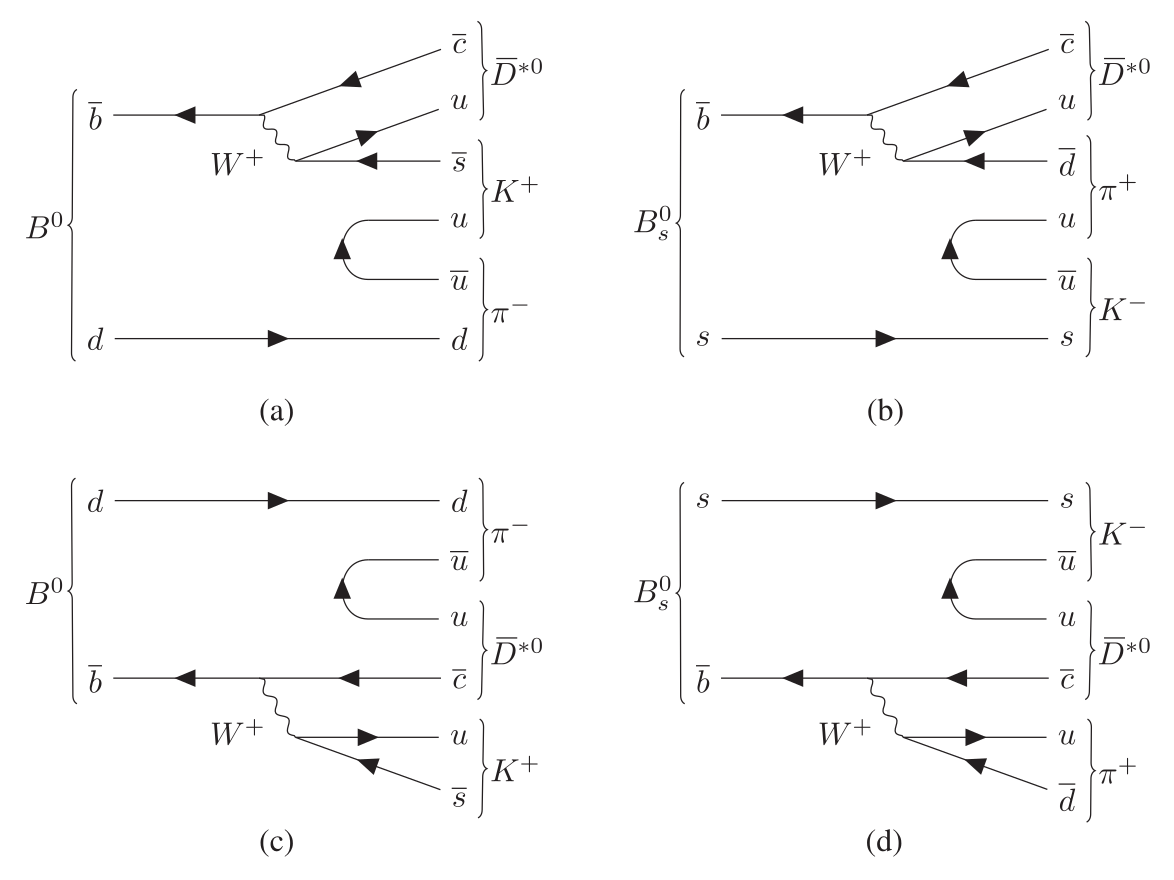
\includegraphics[width=.3\linewidth]{figures/conf/B2DKpi-fig001} \\
    $B \to D\bar{D}$ decays &
    $B \to \bar{D}^* K \pi $ decays \\

    \multicolumn{2}{c}{
      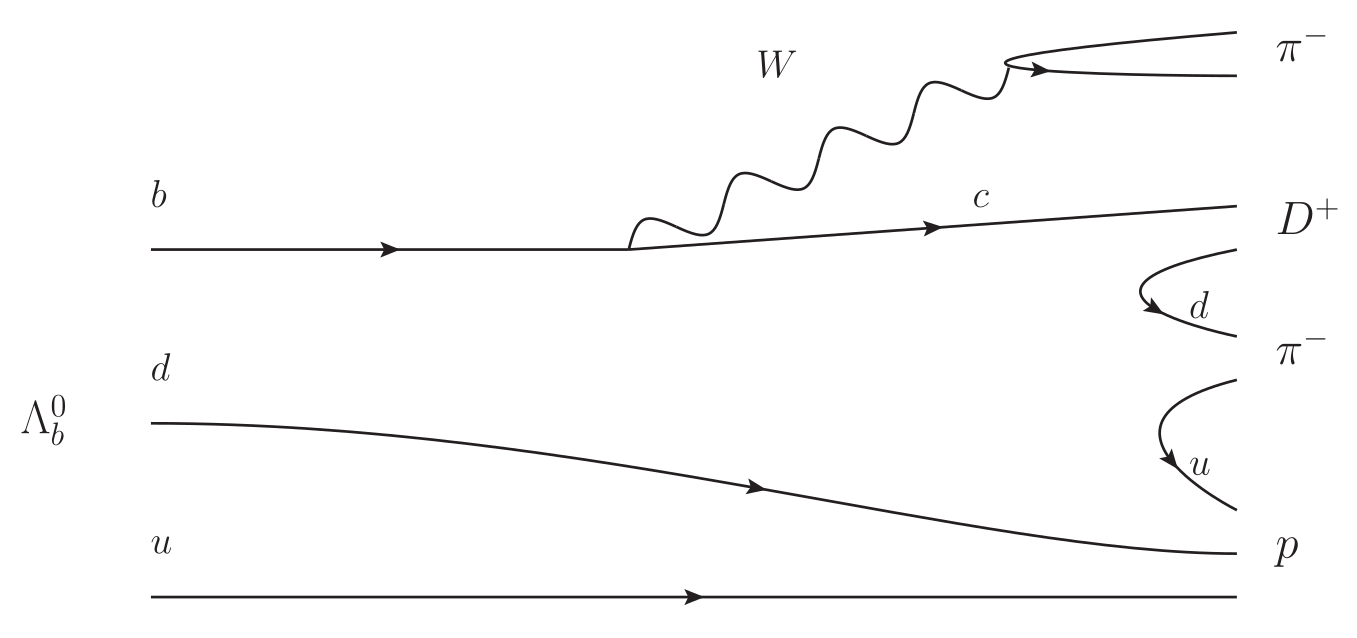
\includegraphics[width=.3\linewidth]{figures/conf/Lb2Dppipi-fig000}
    } \\
    \multicolumn{2}{c}{
      $\Lb\to D^{(*)+} p \pim\pim$ decays
    } \\
  \end{tabular}

  % The process of measurement of branching ratios is the following.
  % First, we need to understand what decays we expect and
  % are interested in. In this case, it's the decays of B mesons
  % into two D mesons, a single D meson, a kaon, and a pion,
  % and the decay of the Lb baryon into a possibly excited D meson,
  % a proton, and two pions.
  % They are all purely hadronic but obviously not the same.
  % The first group is more sensitive to theoretical calculations with 
  % different models.
  % The second group is primarily used for suppression of systematic 
  % uncertainties in future measurements of the CKM gamma angle.
  % And the third group is very sensitive to quark hadronization.
\end{frame}%}}}

\begin{frame}[label=selection]%{{{
  \frametitle{Event selection}

  \begin{itemize}
    \item Cuts on kinematic variables:
      $p_T$, $\eta$, distance from the $pp$ interaction, \ldots,
    \item Cuts on particle identification parameters,
    \item Exclusion of specific troublesome events,
    \item A neural network is used to further improve signal quality.
  \end{itemize}

  \centering \vfill
  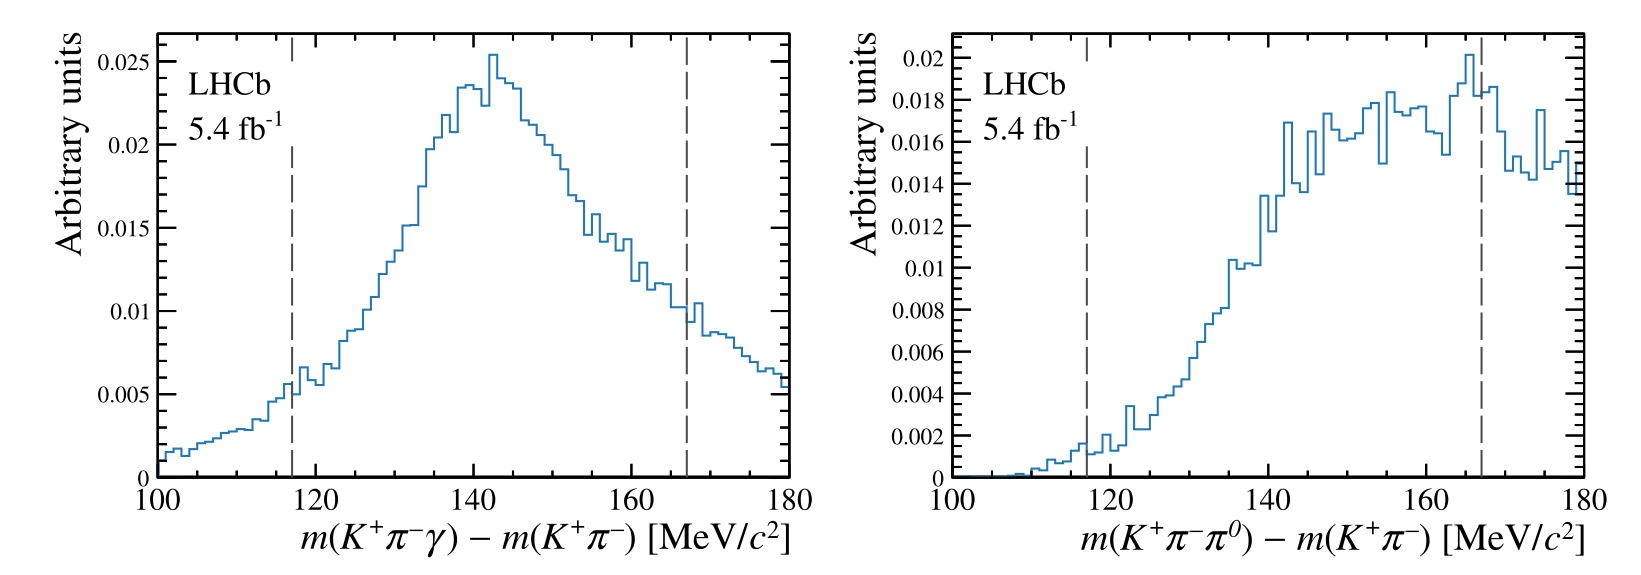
\includegraphics[width=.7\linewidth]{figures/conf/B2DKpi-fig002-pointless}

  % After figuring out the decays the next step is to reasonably extract 
  % them from data. This is performed by applying several cuts on 
  % kinematic variables and particle identification parameters.
  % The detector software reconstructs the whole decay tree including 
  % secondary decays of the D mesons.
\end{frame}%}}}

\begin{frame}[label=model-B2DD]%{{{
  \frametitle{Invariant mass spectrum model and fit:
  $B\to D\bar{D}$ decays}

  \centering
  \def\localwidth{.32\textwidth}
  \parbox{.66\textwidth}{
    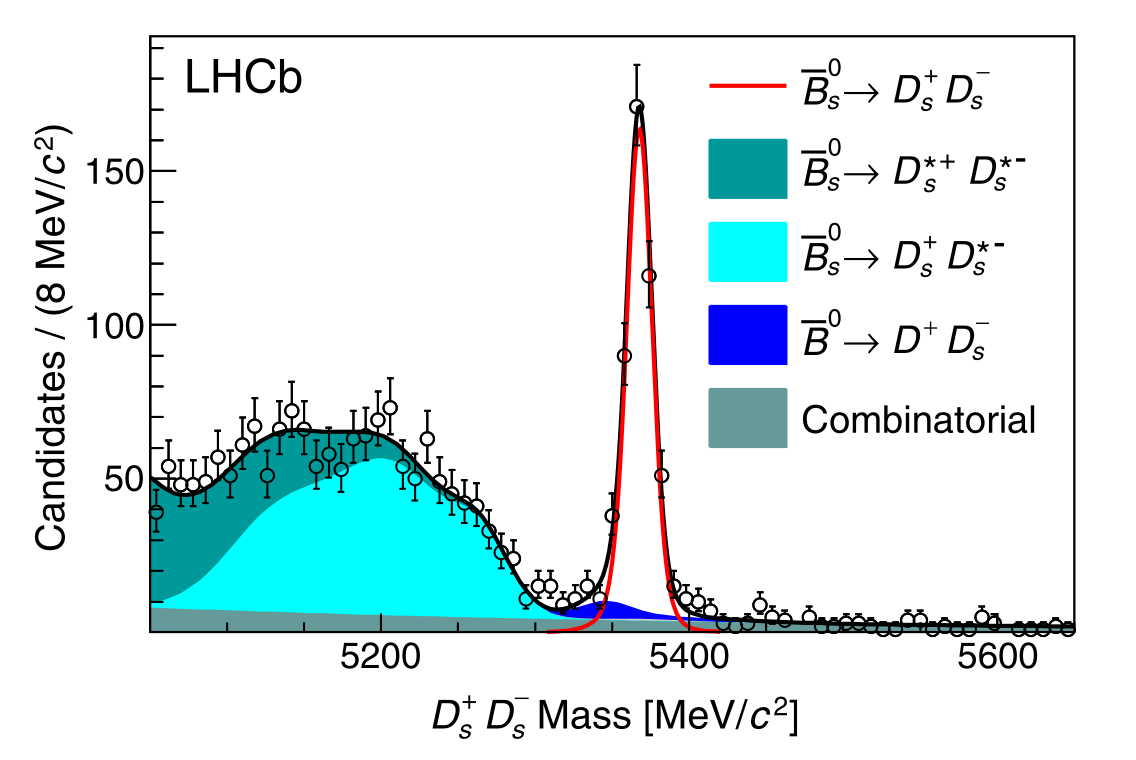
\includegraphics[width=\localwidth]{figures/conf/B2DD-fig002l}
    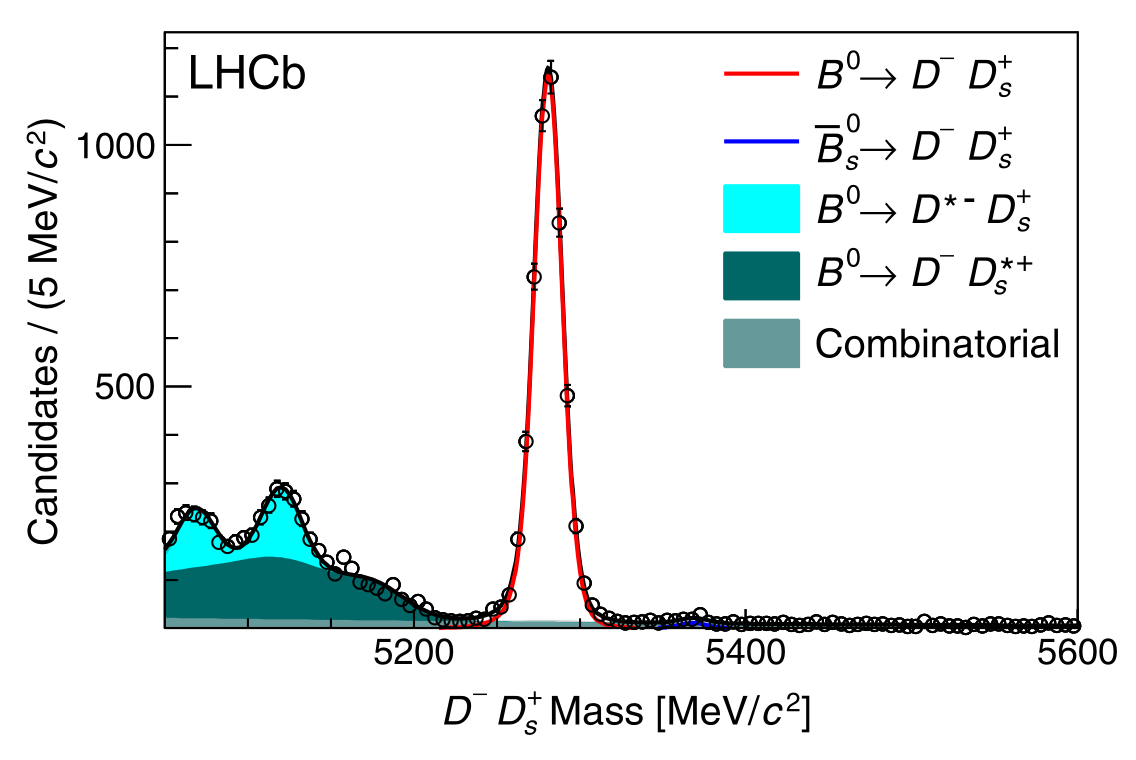
\includegraphics[width=\localwidth]{figures/conf/B2DD-fig002r}
    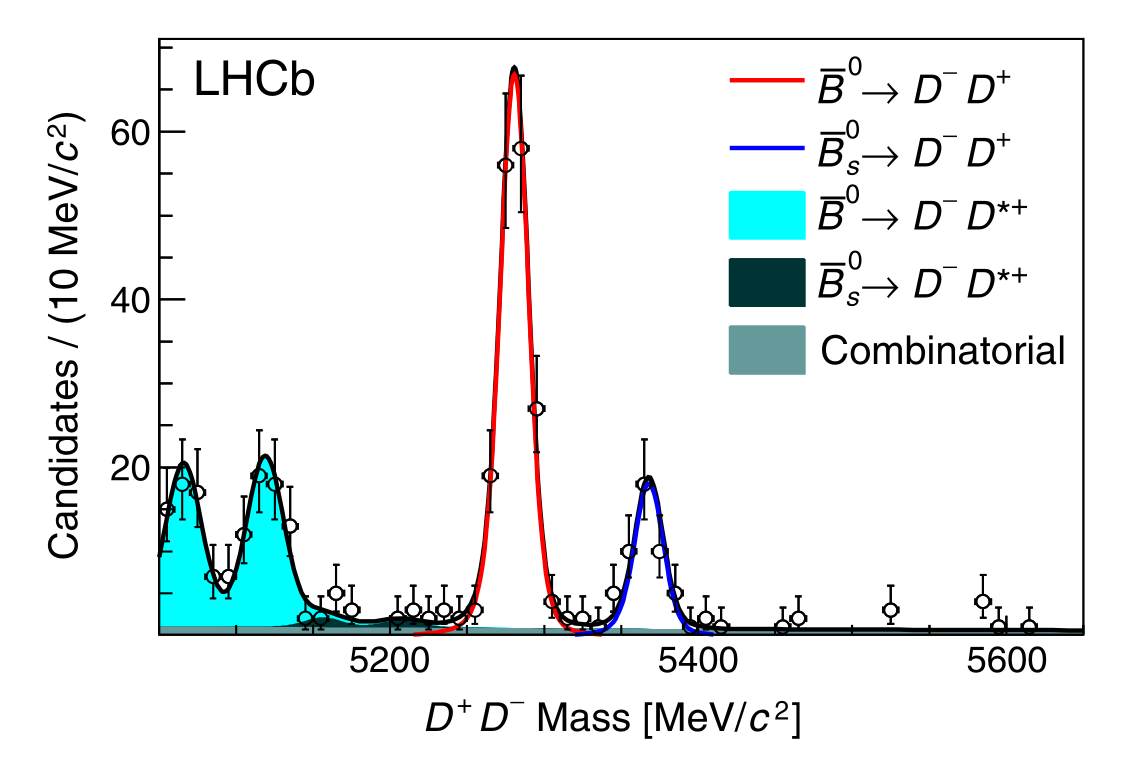
\includegraphics[width=\localwidth]{figures/conf/B2DD-fig004l}
    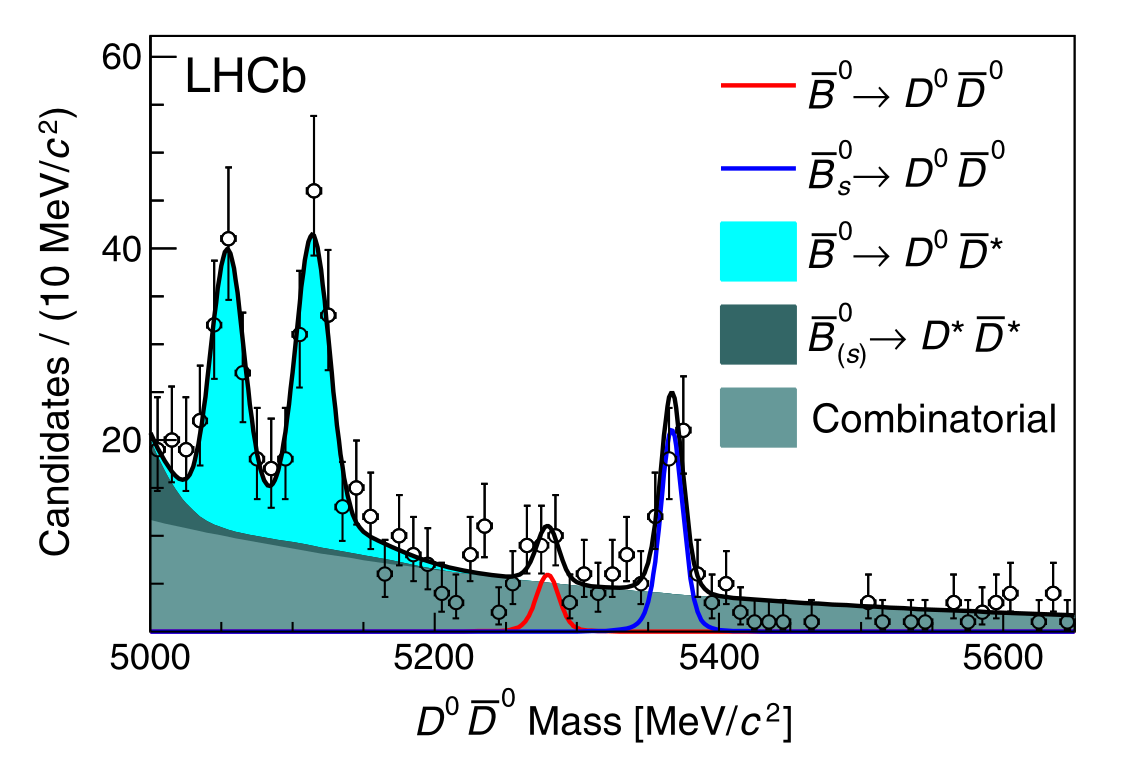
\includegraphics[width=\localwidth]{figures/conf/B2DD-fig004r}
  } \parbox{.33\textwidth}{
    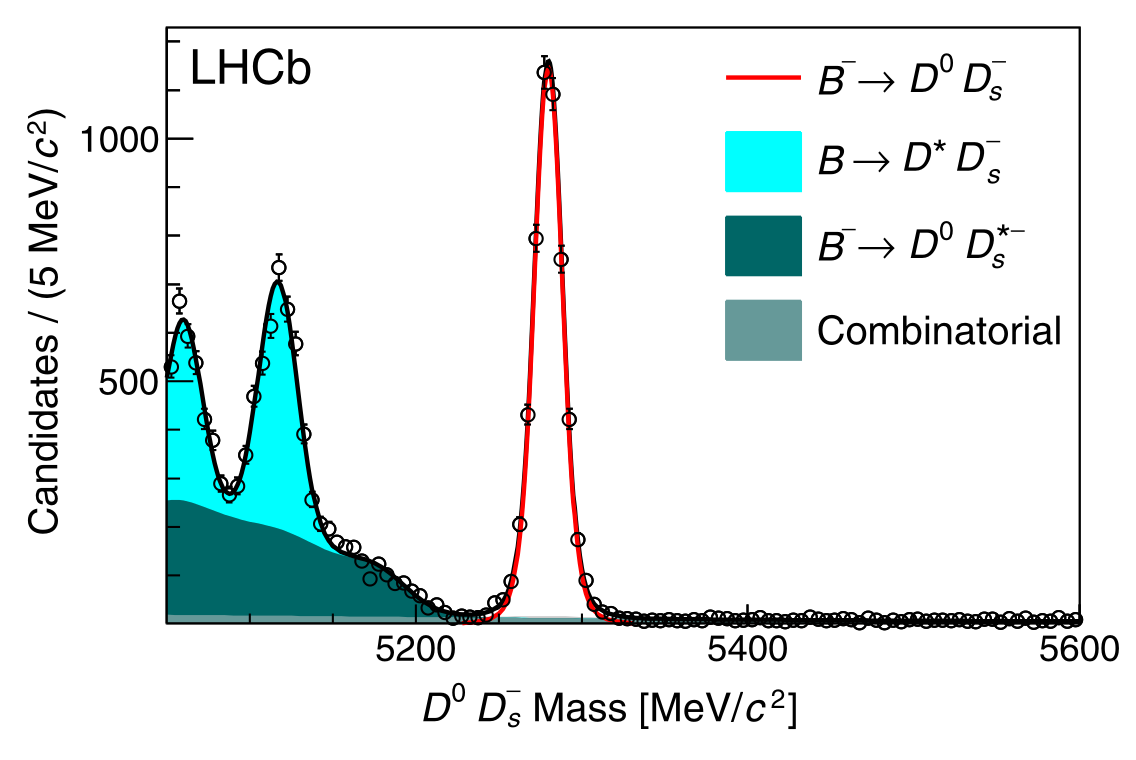
\includegraphics[width=\localwidth]{figures/conf/B2DD-fig005}
    \vskip 2ex
    \centering Normalization
  }

  % During the third step, for each set of final state particles,
  % one constructs a model of their invariant mass spectrum where
  % multiple components should be described based primarily on their 
  % kinematics.
  % Obviously, we are most interested in the main signals, but all the 
  % other shapes should be described just as good for best precision.
  %
  % The simplest shapes are modeled by sample functions like a Gaussian 
  % or a polynomial, while more complex ones are taken from the 
  % simulation and slightly altered to better fit the data.
\end{frame}%}}}

\begin{frame}[label=model-B2DKpi]%{{{
  \frametitle{Invariant mass spectrum model and fit:
  $B\to \bar{D}^*K\pi$ decays}
  \centering

  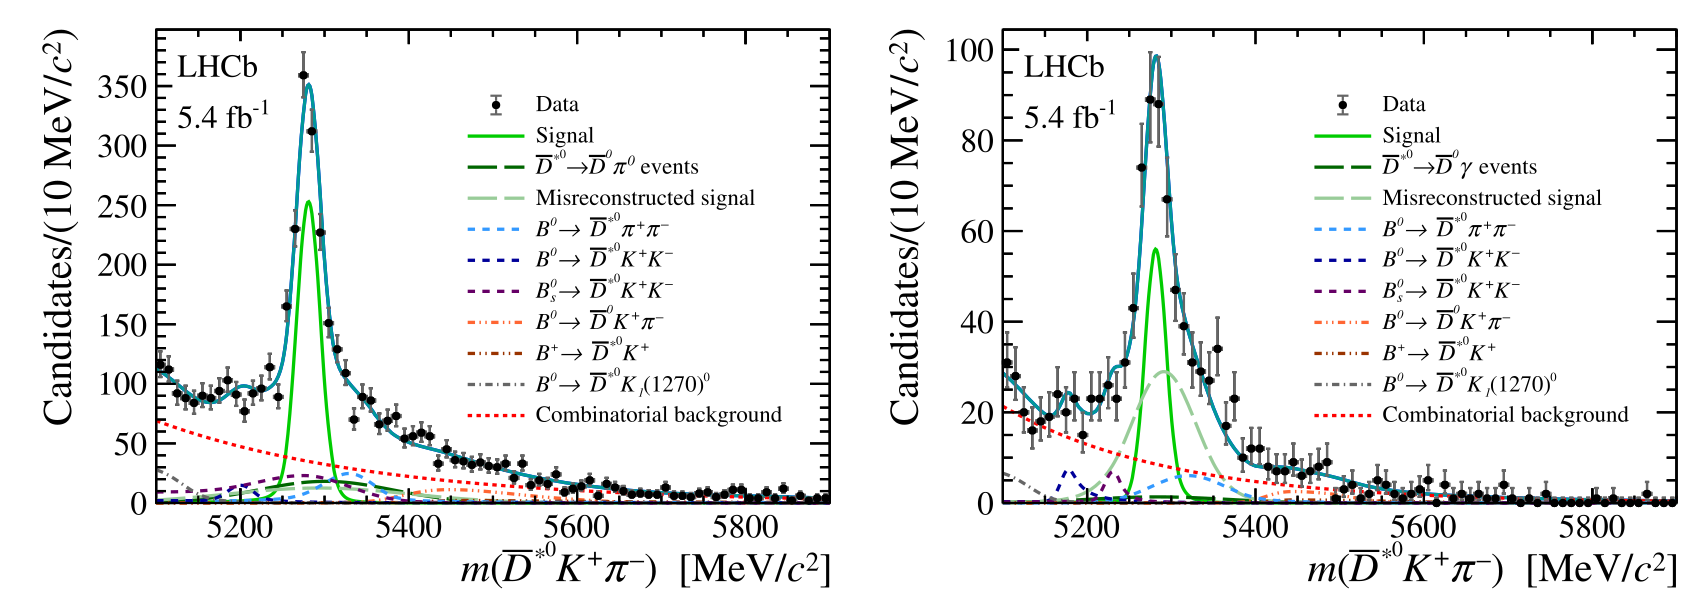
\includegraphics[width=.7\textwidth]{figures/conf/B2DKpi-fig003-top}
  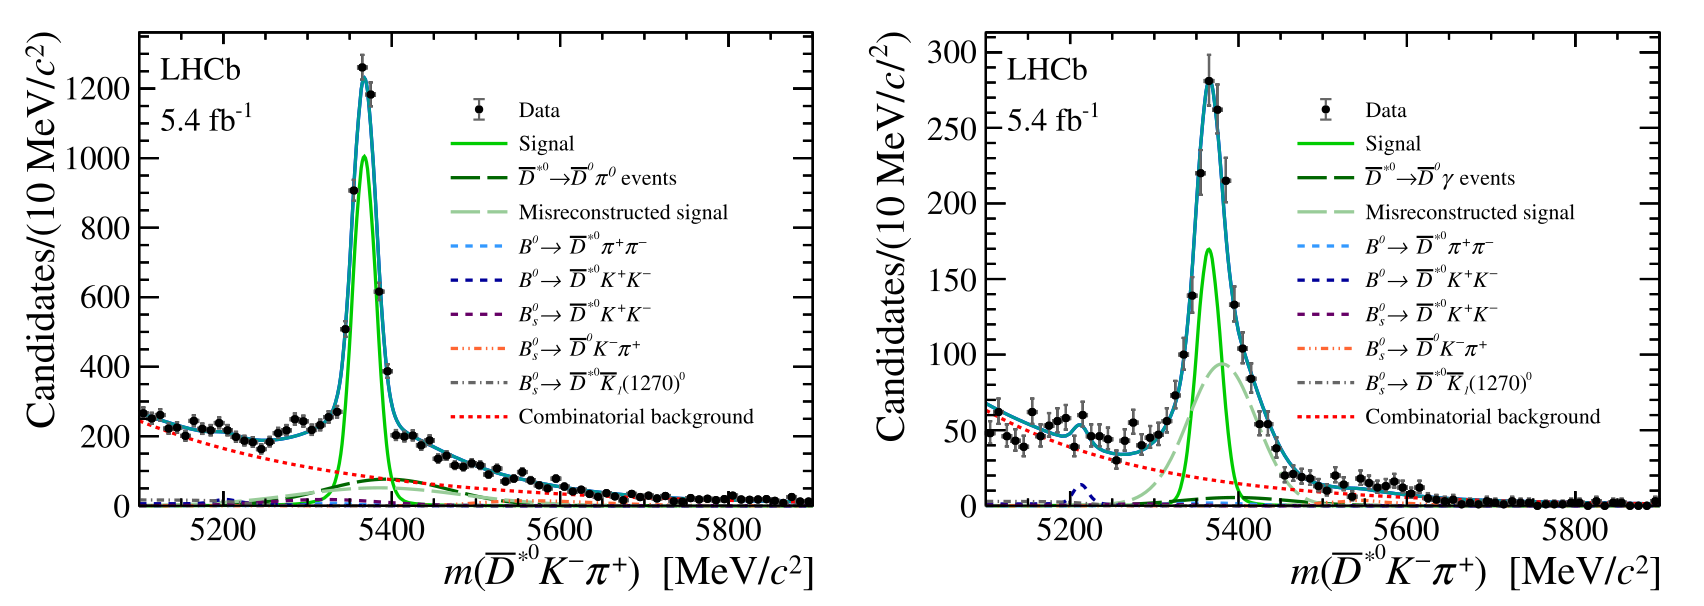
\includegraphics[width=.49\textwidth]{figures/conf/B2DKpi-fig003-mid}
  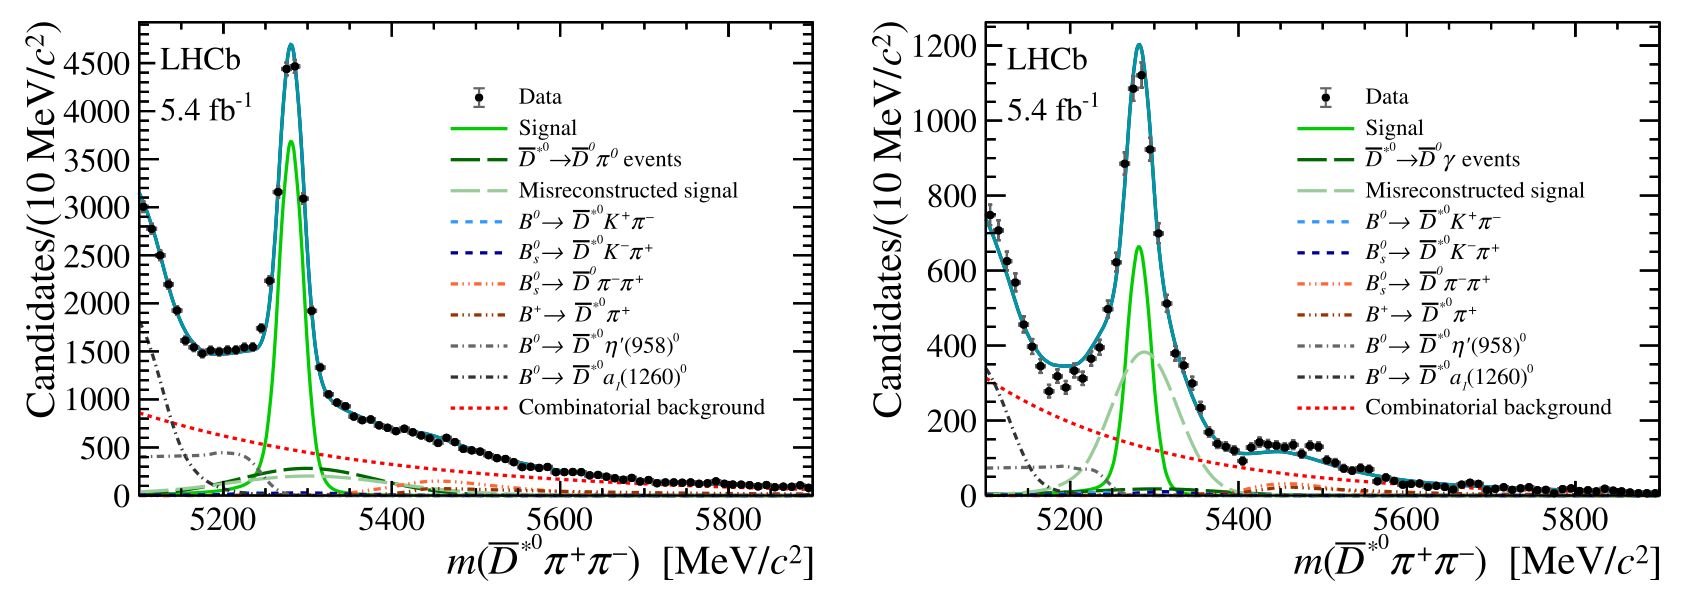
\includegraphics[width=.49\textwidth]{figures/conf/B2DKpi-fig003-bot}

  % When there are too many components, all spectra are fit 
  % simultaneously, and correlations between all of them are included in 
  % the final result.
\end{frame}%}}}

\begin{frame}[label=model-Lb2Dppipi]%{{{
  \frametitle{Invariant mass spectrum model and fit:
  $\Lb \to D^{(*)+} p \pim\pim$ decay}
  \centering

  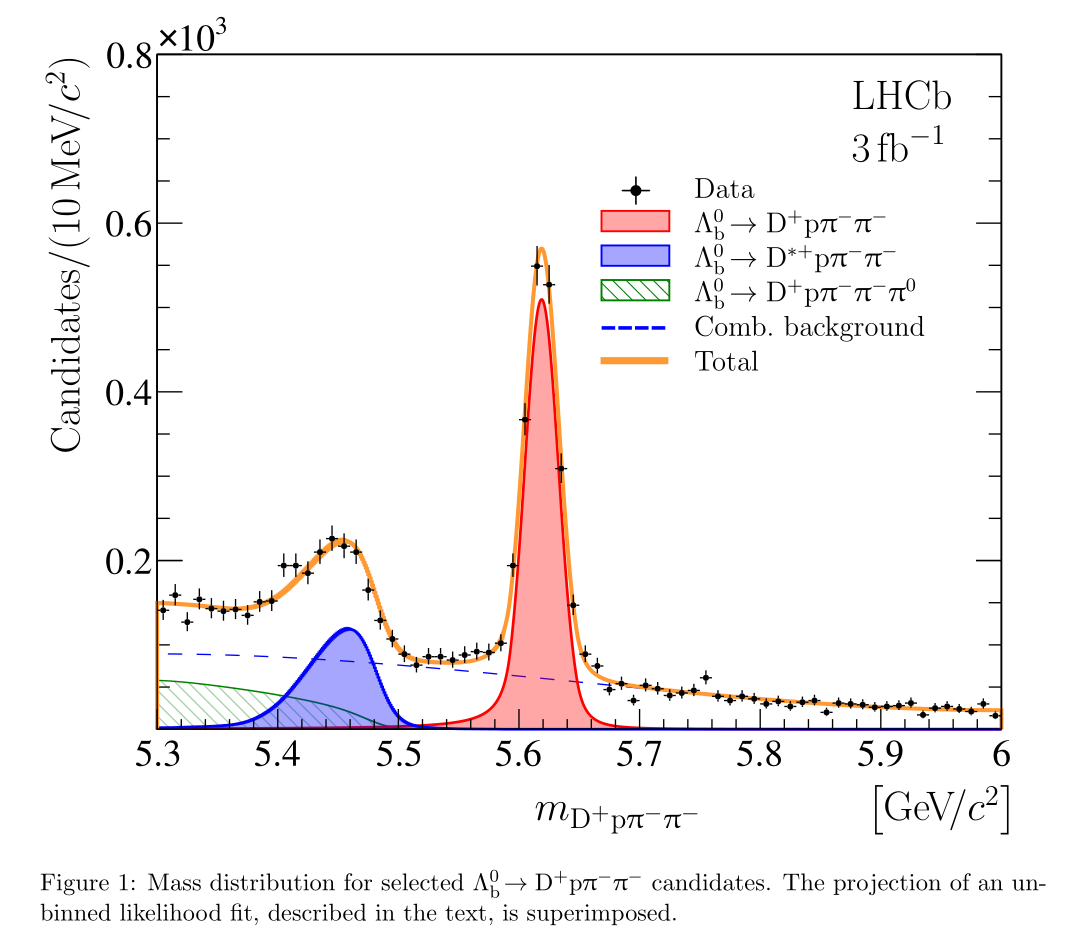
\includegraphics[width=.49\linewidth]{figures/conf/Lb2Dppipi-fig001}
  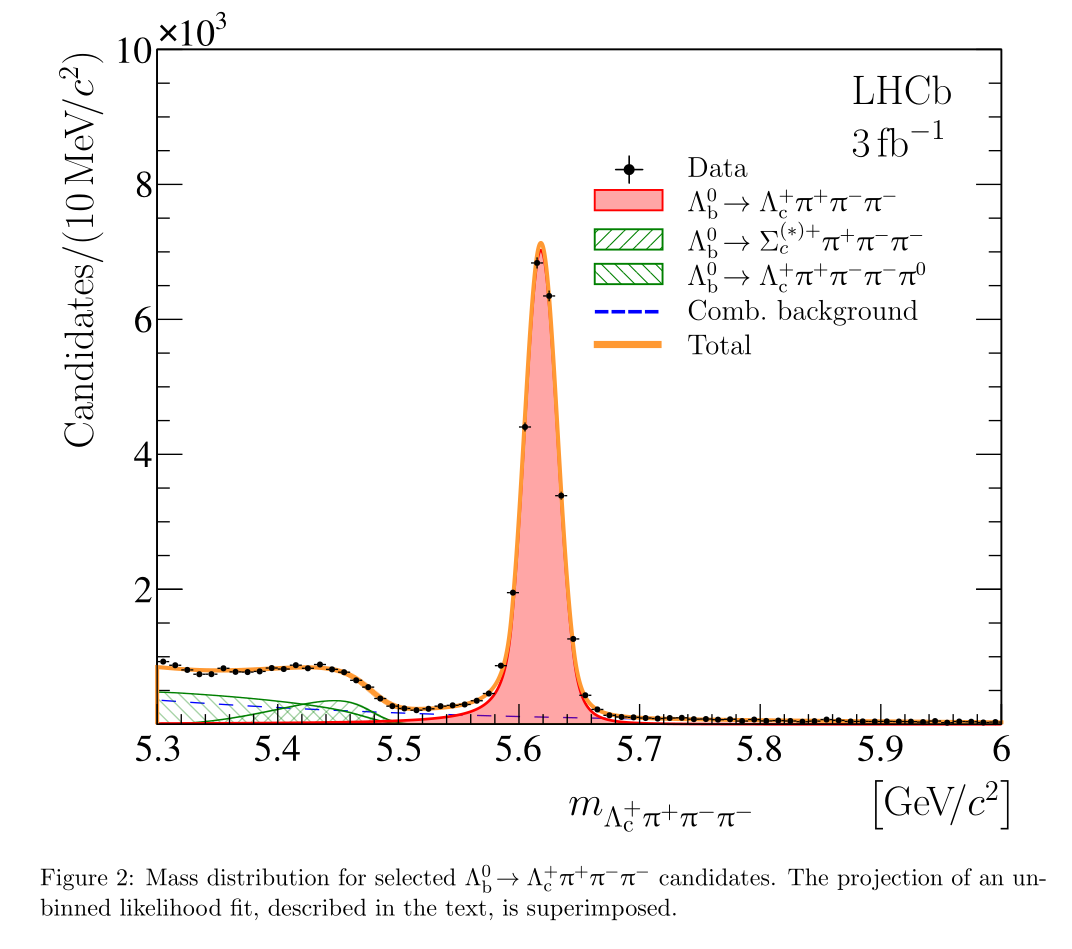
\includegraphics[width=.49\linewidth]{figures/conf/Lb2Dppipi-fig002}
  \parbox{.49\linewidth}{\centering Signal}
  \parbox{.49\linewidth}{\centering Normalization}

  % The decay probabilities are measured relative to each other or 
  % relative to a well-known channel which is called the normalization. 
  % And it requires a separate model and fit.
\end{frame}%}}}

\begin{frame}[label=efficiencies]%{{{
  \frametitle{Corrections for the effects of the selection: efficiencies}

  \centering
  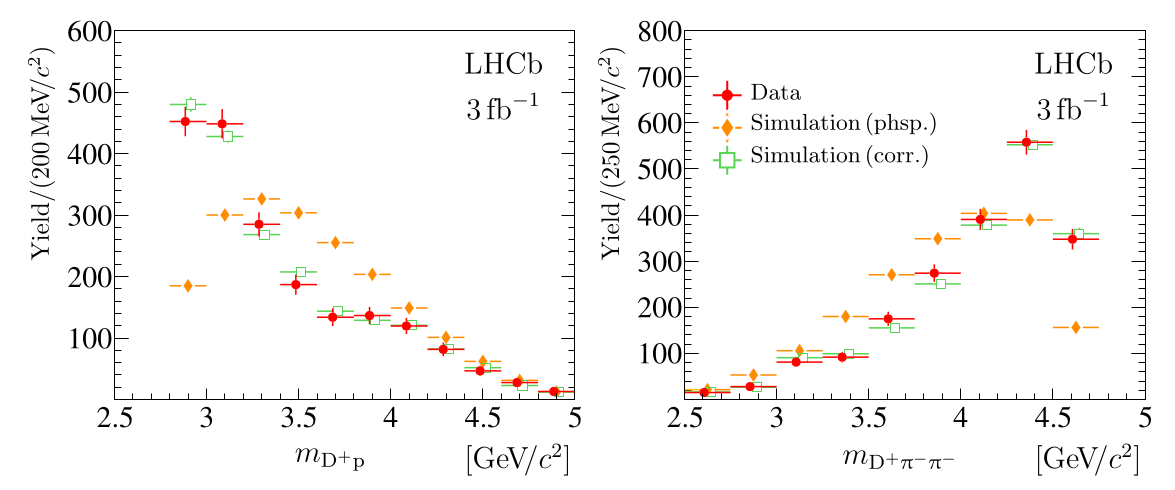
\includegraphics[width=.45\linewidth]{figures/conf/Lb2Dppipi-fig005-1}
  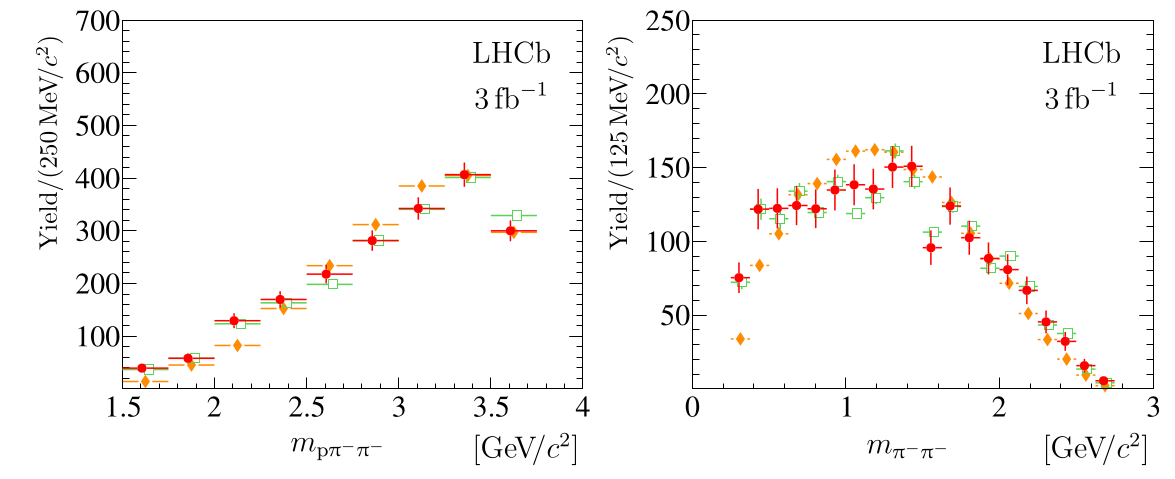
\includegraphics[width=.45\linewidth]{figures/conf/Lb2Dppipi-fig005-2}
  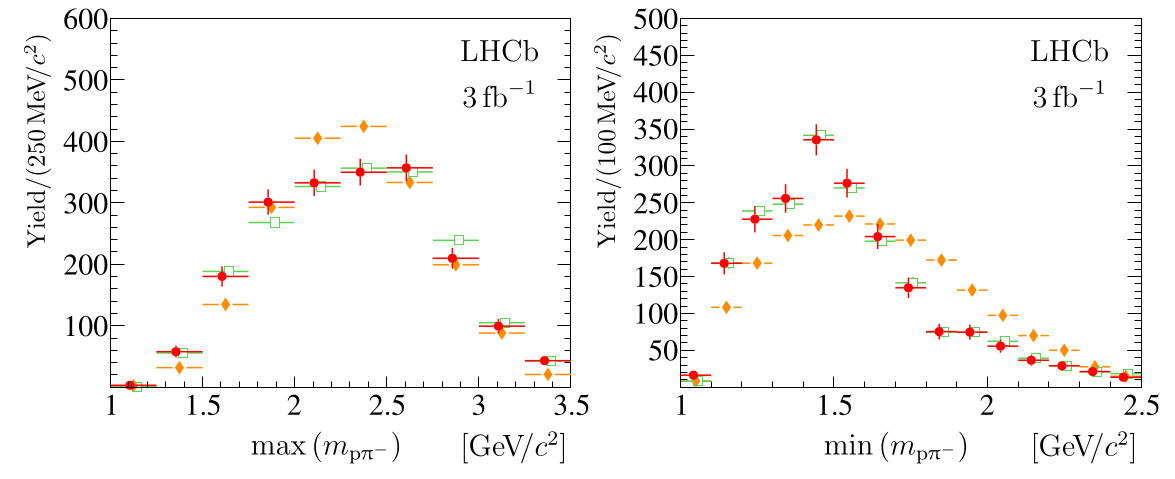
\includegraphics[width=.45\linewidth]{figures/conf/Lb2Dppipi-fig005-3}
  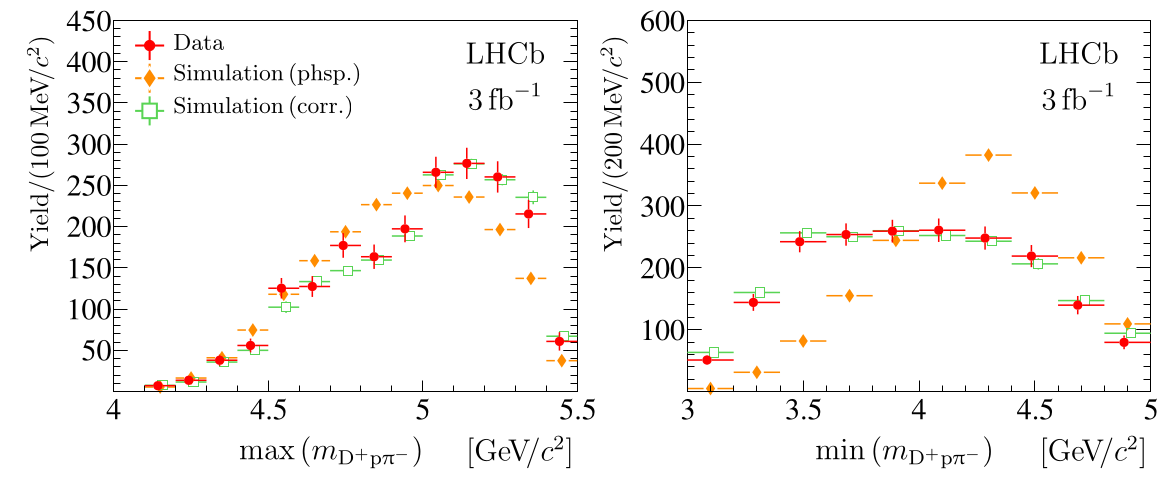
\includegraphics[width=.45\linewidth]{figures/conf/Lb2Dppipi-fig006-1}

  % The fit results are signal yields in each specific decay channel. 
  % The channels may behave differently when subjected to the chosen 
  % event selection procedures. And the fourth step deals with this. All 
  % the selection criteria are applied to the simulation, and the event 
  % counts before and after the selection are then used to correct the 
  % signal yields.
  % When the simulation does not perfectly represent the data, it is 
  % initially corrected itself for better representation and hence 
  % precision.
\end{frame}%}}}

\begin{frame}[label=systematics]%{{{
  \frametitle{Systematic uncertainties}

  The largest sources if systematic uncertainty are
  \begin{itemize}
    \item the fitting model,
    \item the approach to combining results with different secondary 
      decays,
    \item the finite size of the simulation,
    \item the approach to excluding unwanted events like duplicates,
    \item the limited knowledge of constants.
  \end{itemize}

  \vfill

  The total systematic uncertainty of the branching ratios ranges from 
  3\% to 12\% for different decays.

  % The fifth and final step is to estimate systematic uncertainties 
  % caused by the whole chosen measurement approach.
  % The largest sources if systematic uncertainty are
  % - the fitting model
  % - the approach to combining results with different secondary decays
  % - the finite size of the simulation
  % - the approach to excluding unwanted events like duplicates
  % - the limited knowledge of constants
  % The total systematic uncertainty of the branching ratios ranges from 
  % 3 percent to 12 for different decays.
\end{frame}%}}}

\begin{frame}[label=results]%{{{
  \frametitle{Results: branching ratios of the $B$ and $\Lb$ decays}

  \parbox{.45\linewidth}{
    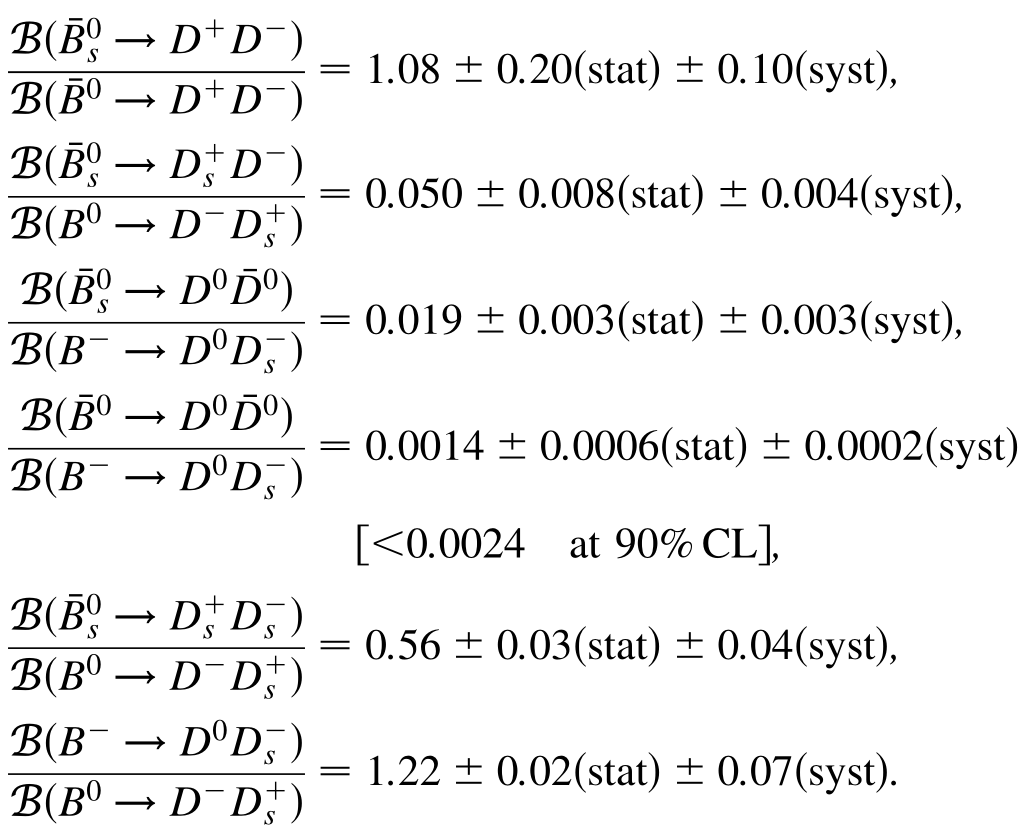
\includegraphics[width=\linewidth]{figures/conf/B2DD-txt001-results}
  } \hfill \parbox{.54\linewidth}{
    \centering
    \footnotesize

    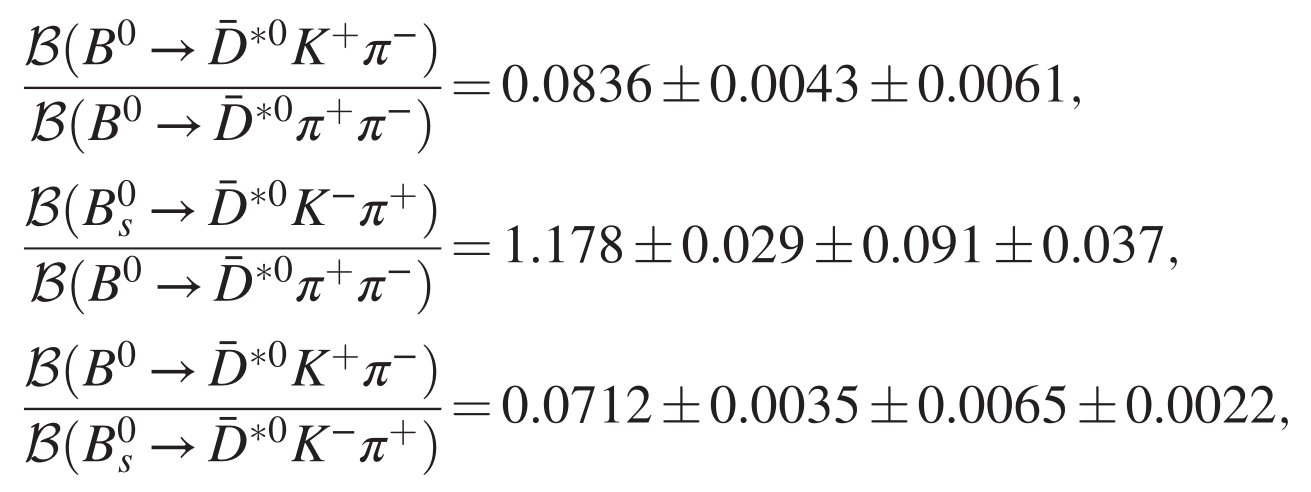
\includegraphics[width=.45\textwidth]{figures/conf/B2DKpi-txt001-results}

    $$\begin{aligned} %\mathcal{R}_{\Dp} =
    \frac{\mathcal{B}\left(\Lb\to\Dp p\pim\pim\right)}
    {\mathcal{B}\left(\Lb\to\Lc\pip\pim\pim\right)}
    \times
    \frac{\mathcal{B}\left(\Dp\to\Km\pip\pip\right)}
    {\mathcal{B}\left(\Lc\to p\Km\pip\right)}
      = \\ = (5.35\pm0.21\pm0.16)\%
    \end{aligned}$$

    $$\begin{aligned}%\mathcal{R}_{\Dstarp} =
    \frac{\mathcal{B}\left(\Lb\to\Dstarp p\pim\pim\right)}
    {\mathcal{B}\left(\Lb\to\Dp p\pim\pim\right)}
    \times
    \mathcal{B}\left(\Dstarp\to\Dp\piz,\ \Dp\gamma\right)
    = \\ = (61.3\pm4.3\pm4.0)\% \end{aligned}$$
  }
\end{frame}%}}}

\begin{frame}[label=conclusion]%{{{
  \frametitle{Conclusion}

  \begin{itemize}
    \item First observation of
      $\bar{B}_s^0 \to D^+ D^-$,
      $\bar{B}_s^0 \to D_s^+ D^-$,
      $\bar{B}_s^0 \to D^0 \bar{D}^0$,
      $\Lb\to\Dp p\pim\pim$,
      $\Lb\to\Dstarp p\pim\pim$.
    \item Measurements of
      $\bar{B}_s^0 \to D_s^+ D_s^-$,
      ${B}_s^- \to D^0 D_s^-$.
    \item The measurements of the $B\to D \bar{D}$ decays favor the 
      perturbative QCD predictions, not phenomenological ones.

    \item The studied $B\to \bar{D}^* K \pi$ decays have large 
      significances (over $5\sigma$).
      \\ The results and the extracted final state particle 
      distributions will be very useful for future CKM~$\gamma$ 
      angle measurements.

    \item BRs of the $\Lb$ baryon give a very similar ratio of $D$ and 
      $D^*$ mesons compared to $ee$ annihilation.
      The hadronization must be the very similar.
  \end{itemize}

  \pause

  \centering \vfill
  \hfill Thank you! \hfill\null
\end{frame}%}}}

\end{document}

\begin{frame}[label=B2DD-intro]%{{{
  \frametitle{$B \to D \bar{D}$ decays: Feynman diagrams}
  \centering

  \parbox{.32\linewidth}{\centering (a) Tree diagrams}
  \parbox{.32\linewidth}{\centering (b) $W$-exchange diagrams}
  \parbox{.32\linewidth}{\centering (c) Penguin diagrams}
  \vskip 2ex
  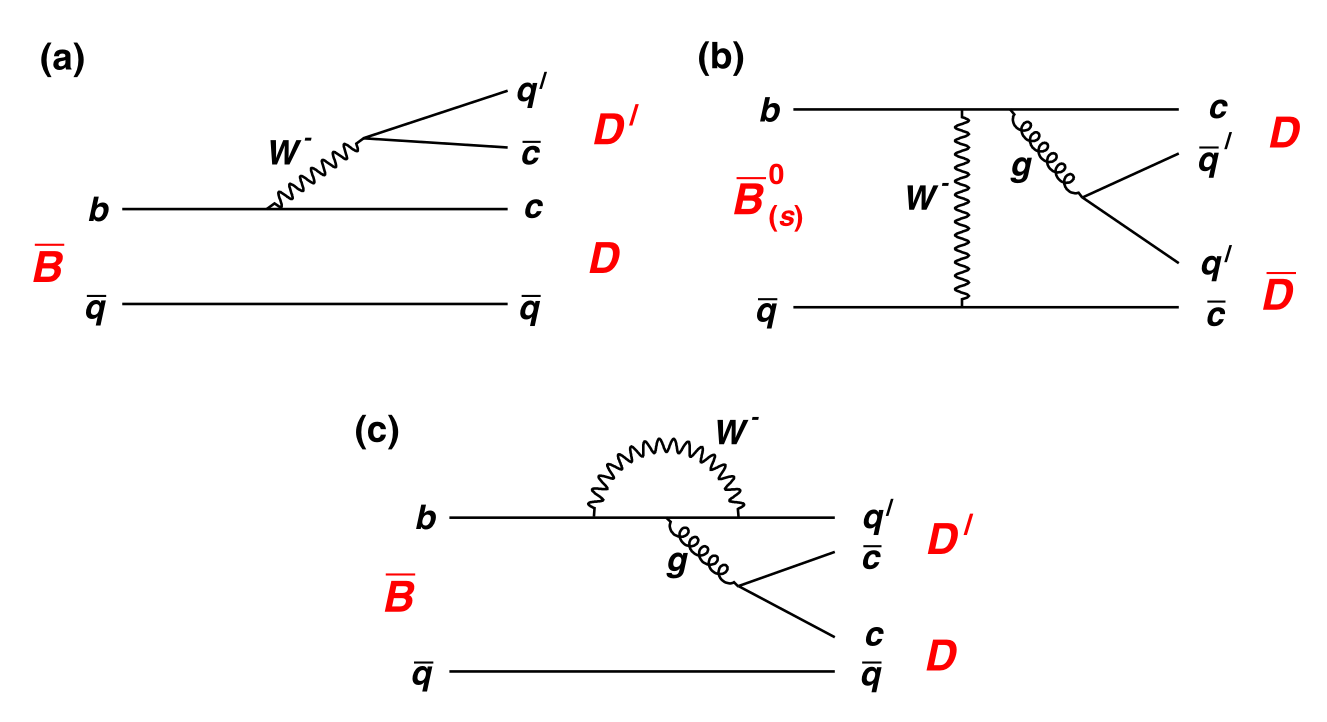
\includegraphics[width=.7\linewidth]{figures/conf/B2DD-fig001}

  % Notes:
  %
  % Kaon and pion eff. are calc. based on reweighted data.
  %
  % Evt. reco: D decays, D mass constr.
  % Strange cross-feed veto of D events that look similar to Ds or Lc.
  % Cut on D meson vertex displacement fit quality.
  % BDT recognition against non-DD B decays with D pi.
  %
  % Zero understanding of what they are talking about.
\end{frame}%}}}

\begin{frame}[label=B2DD-selection]%{{{
  \frametitle{$B\to D\bar{D}$ event selection}

  \begin{itemize}
    \item Detector selection:
      $p_T$,
      distance from $pp$ interaction,
      secondary vertices.

    \item $D$ mesons are reconstructed in
      decays to $K$, $\pi$ and require an extra vertex.
      % $\Dz\to\Km\pip$, $\Dz\to\Km\pip\pim\pip$,
      % $\Dp\to\Km\pip\pip$,
      % $\Dsubsp\to\Kp\Km\pip$.
      %A mass constraint is also applied.

    \item Vetoes on $\Km\pip h^+$ with ambiguous $h^+$:
      $\Kp$, $\pip$, $p$.

    \item A BDT is used to improve quality of signals.

    \item Efficiencies: simulation, calibration data.
      Also used for specific backgrounds.
  \end{itemize}

  \centering
  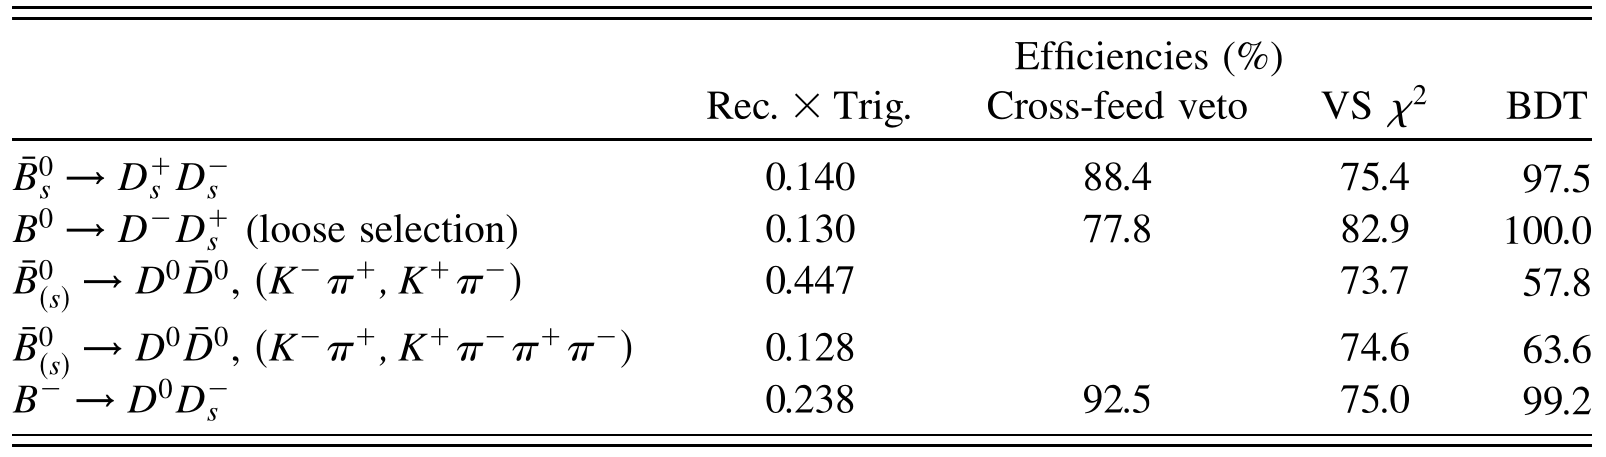
\includegraphics[width=\linewidth]{figures/conf/B2DD-tab001}
\end{frame}%}}}

\begin{frame}[label=B2DD-fit-1]%{{{
  \frametitle{$B\to D\bar{D}$ models and fit results}

  \begin{itemize}
    \item Signals are modified Gaussians
      and accommodate for both resolution and radiation.
    \item Sensitive parameters are fixed to simulation.
    \item $D^*$ background shapes are derived from the simulation.
    \item Combinatorial background is described by an exponent.
  \end{itemize}

  \centering
  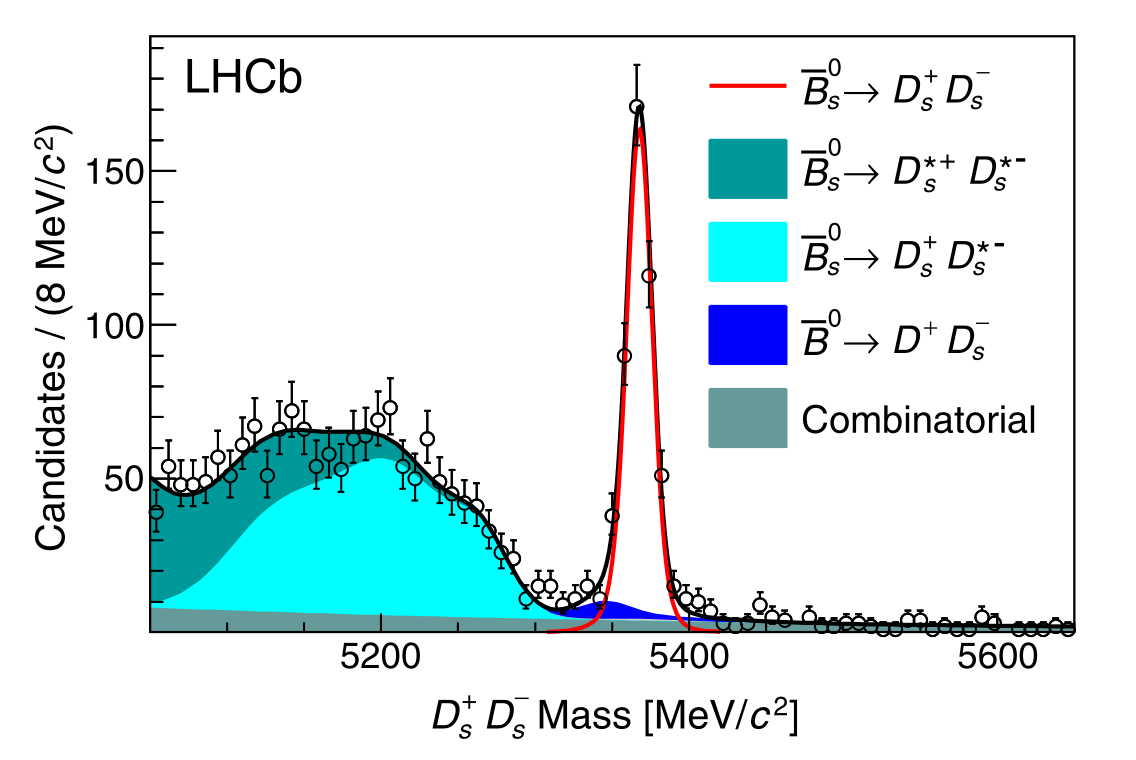
\includegraphics[width=.49\linewidth]{figures/conf/B2DD-fig002l}
  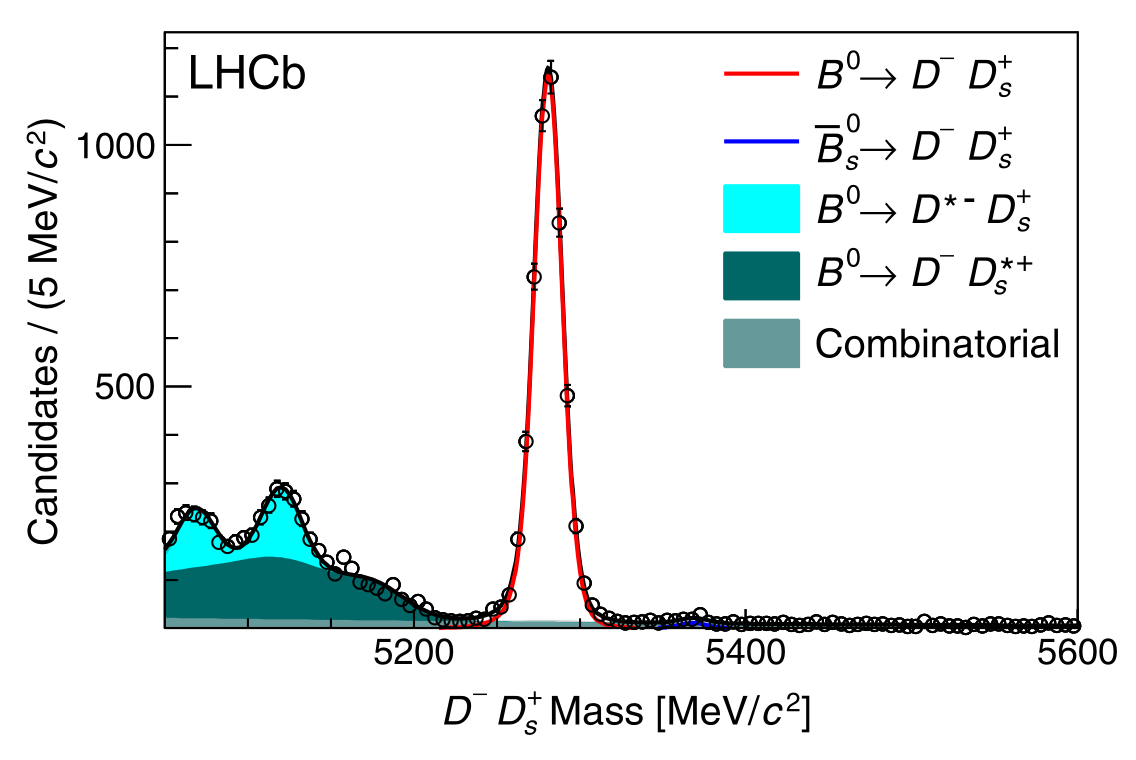
\includegraphics[width=.49\linewidth]{figures/conf/B2DD-fig002r}
\end{frame}%}}}

\begin{frame}[label=B2DD-fit-2]%{{{
  \frametitle{$B\to D\bar{D}$ models and fit results}

  \centering
  \def\localwidth{.32\textwidth}
  \parbox{.66\textwidth}{
    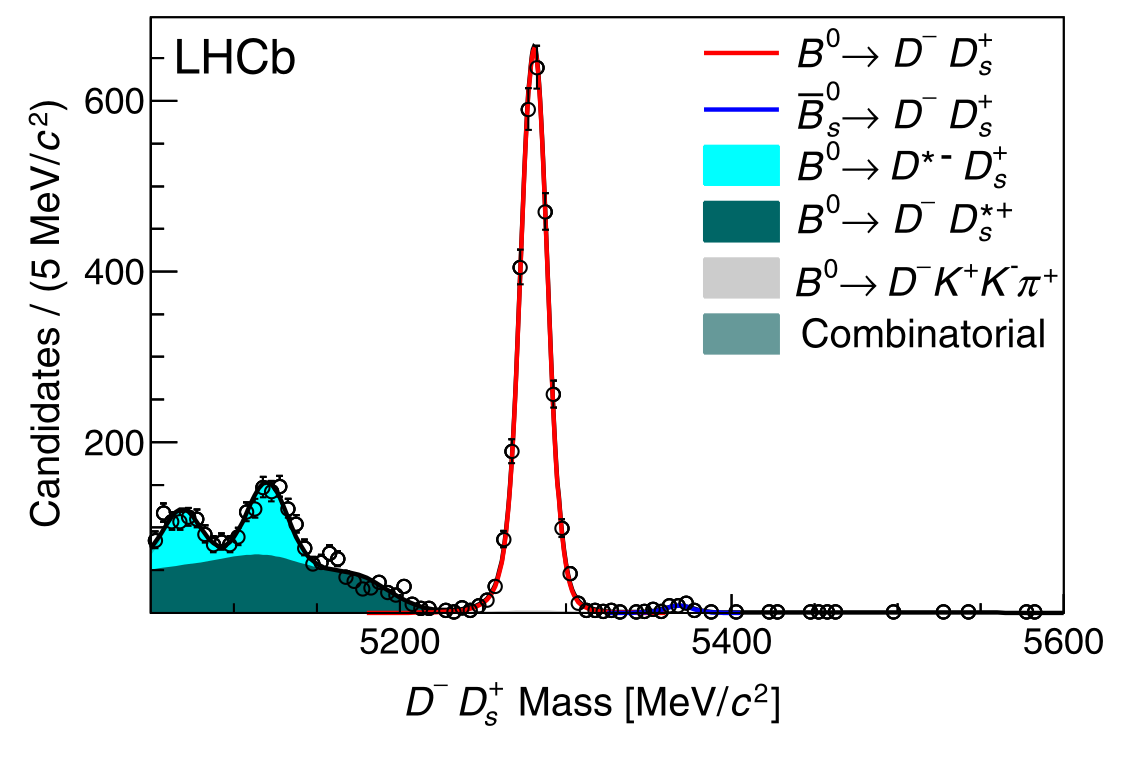
\includegraphics[width=\localwidth]{figures/conf/B2DD-fig003l}
    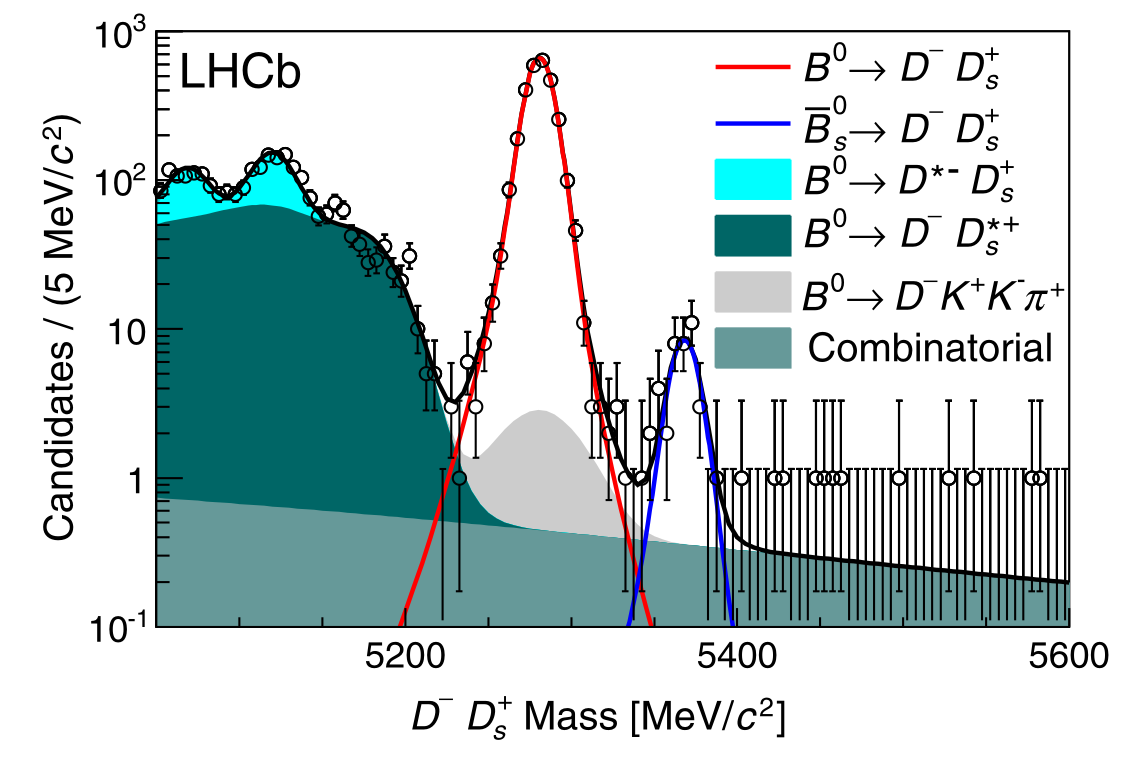
\includegraphics[width=\localwidth]{figures/conf/B2DD-fig003r}
    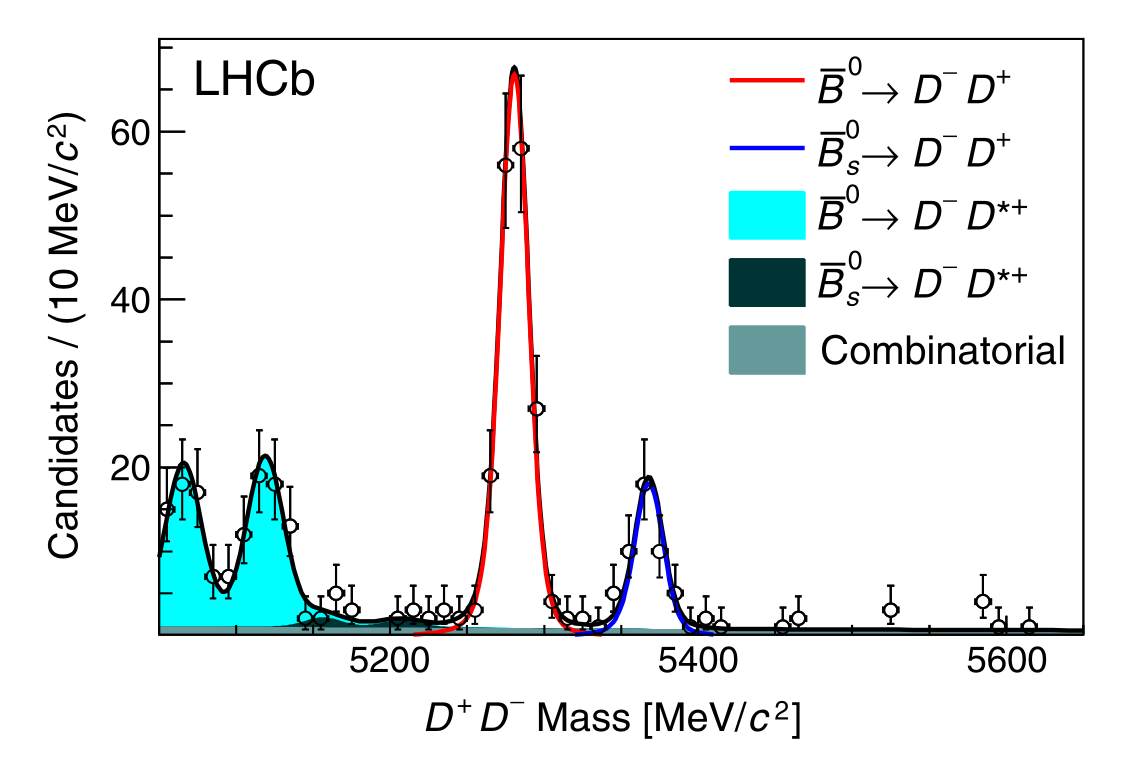
\includegraphics[width=\localwidth]{figures/conf/B2DD-fig004l}
    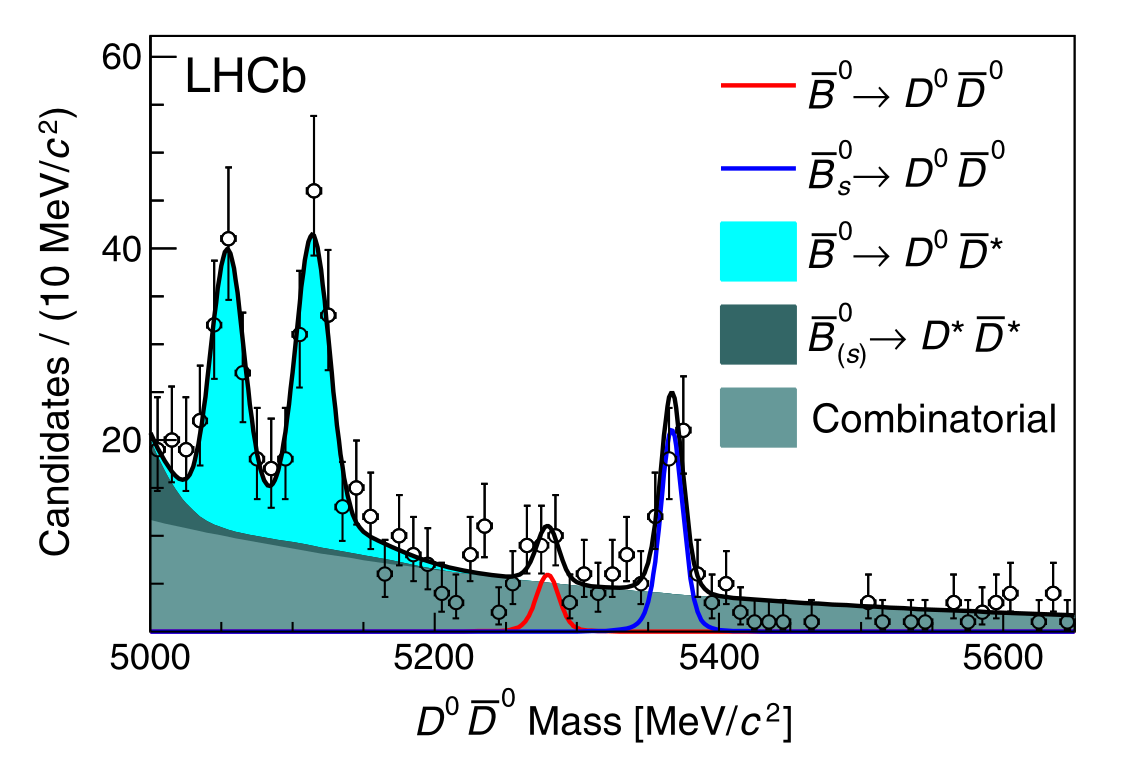
\includegraphics[width=\localwidth]{figures/conf/B2DD-fig004r}
  } \parbox{.33\textwidth}{
    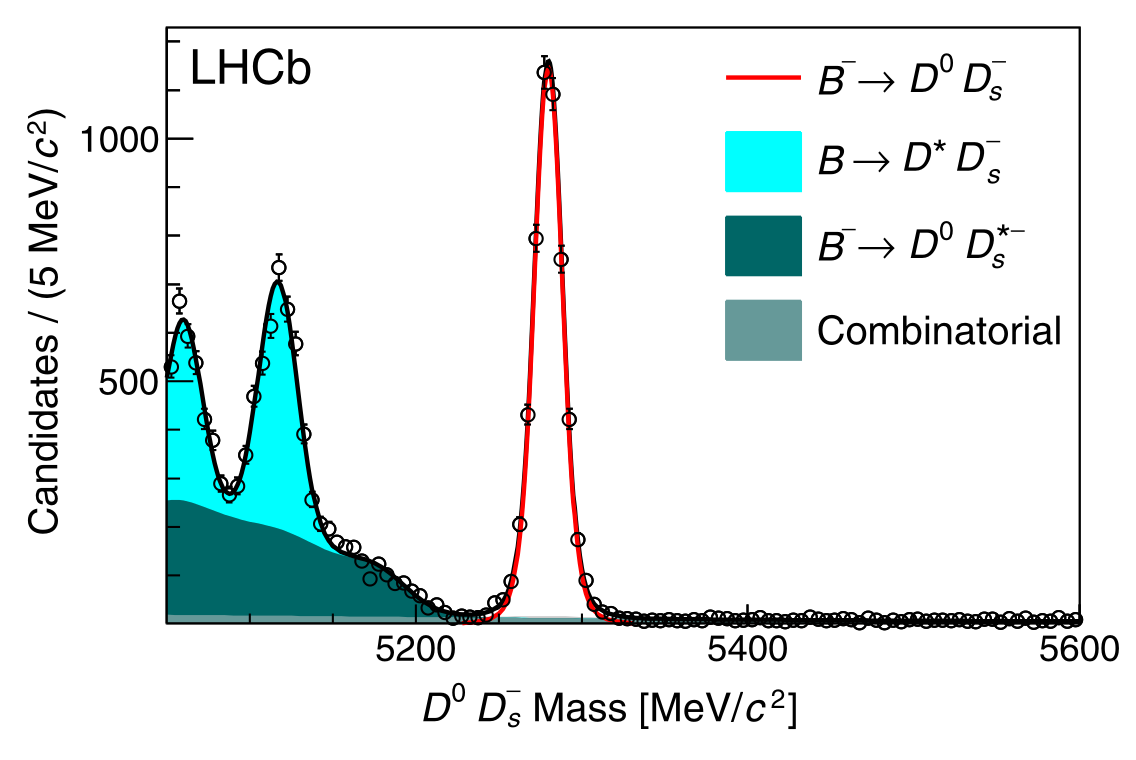
\includegraphics[width=\localwidth]{figures/conf/B2DD-fig005}
    \vskip 2ex
    \centering Normalization
  }
\end{frame}%}}}

\begin{frame}[label=B2DD-syst]%{{{
  \frametitle{$B\to D\bar{D}$ systematic uncertainties}

  The final branching ratios require the yields,
  relative efficiencies, and factorization ratios.

  \vfill \centering
  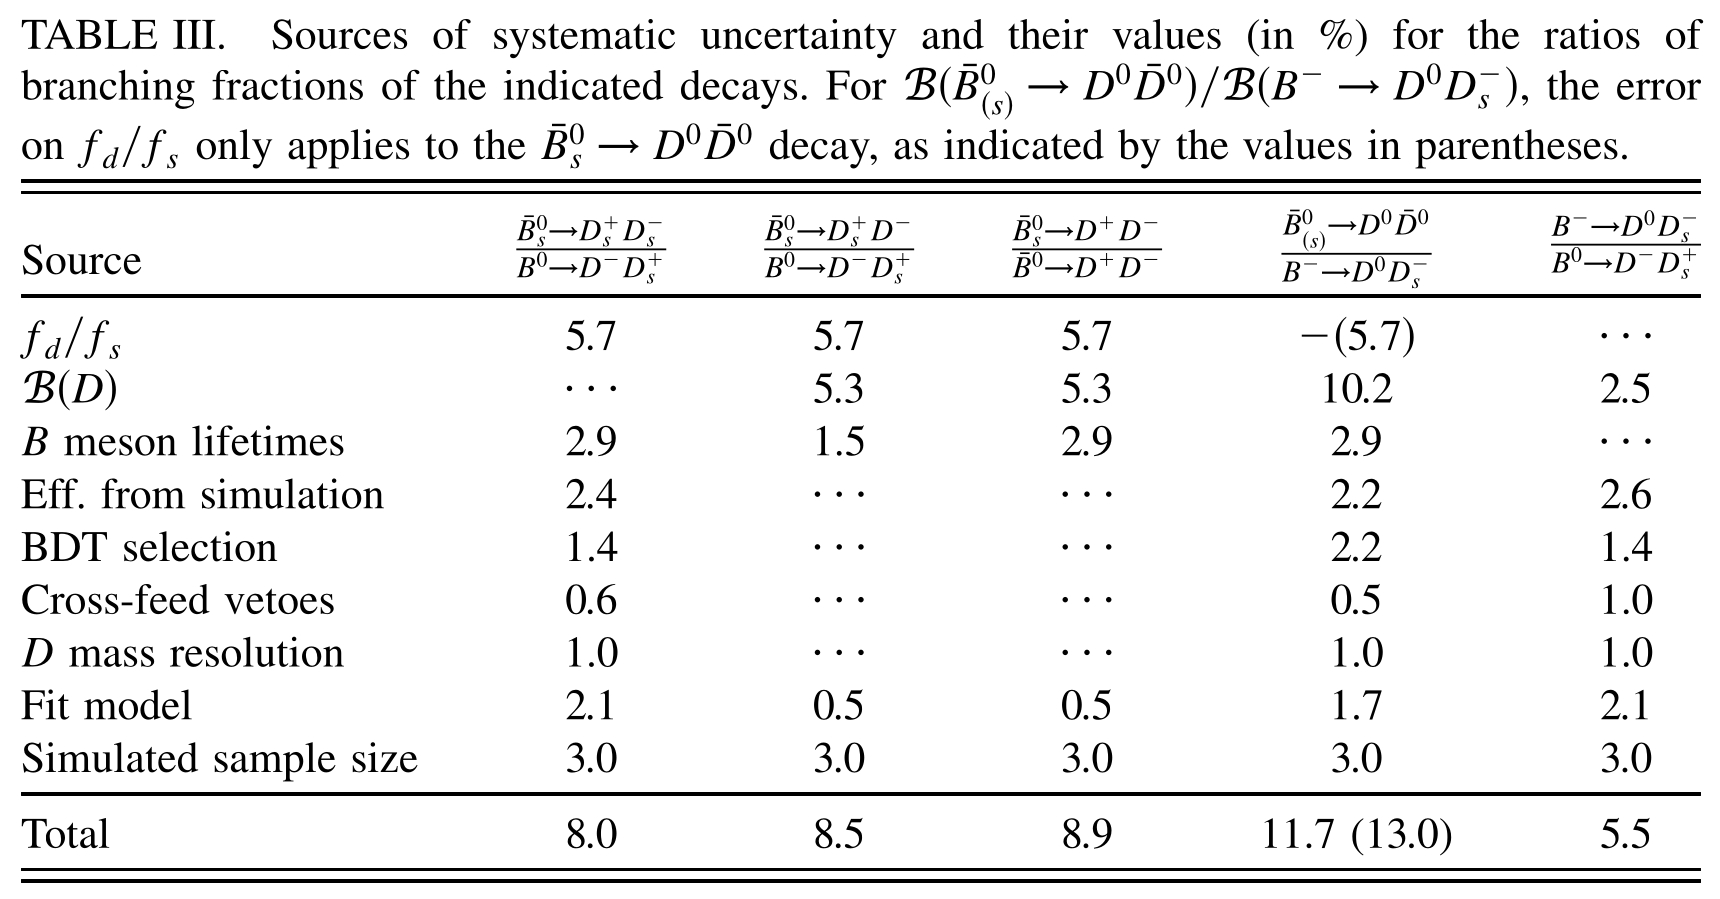
\includegraphics[width=.7\linewidth]{figures/conf/B2DD-tab003}
\end{frame}%}}}

\begin{frame}[label=B2DD-results]%{{{
  \frametitle{$B\to D\bar{D}$ branching ratios}

  \parbox{.45\linewidth}{
    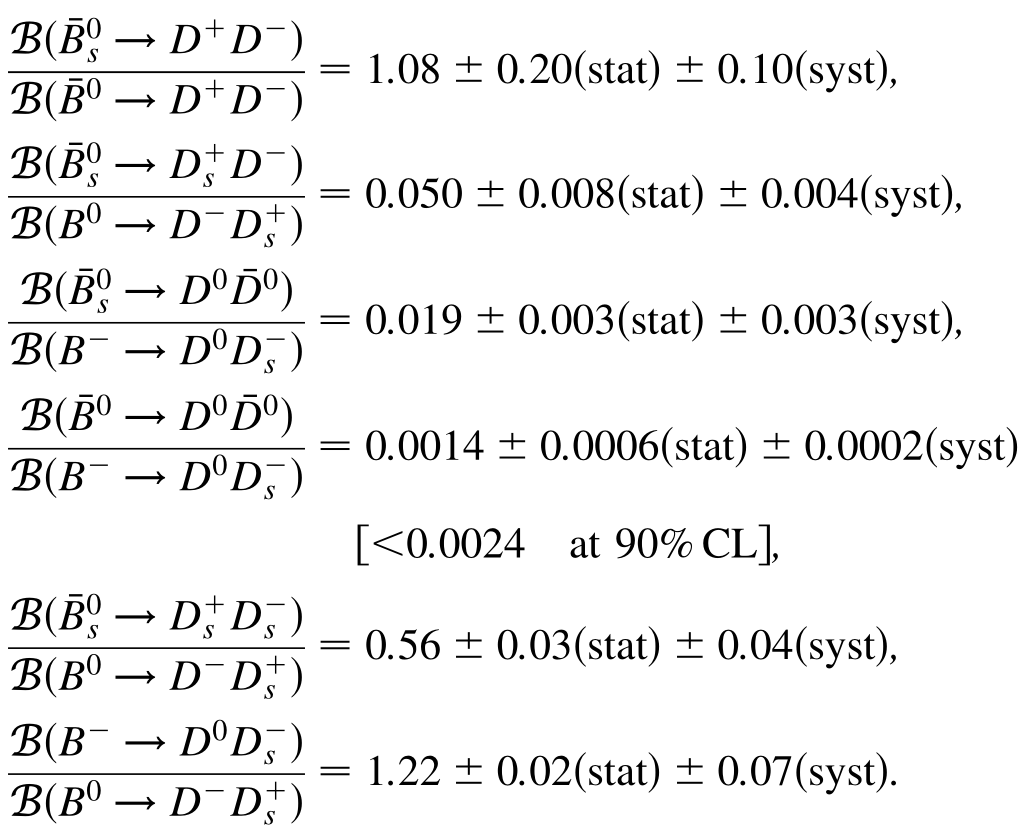
\includegraphics[width=\linewidth]{figures/conf/B2DD-txt001-results}
  } \hfill \parbox{.5\linewidth}{
    \begin{itemize}
      \item First observation of
        $\bar{B}_s^0 \to D^+ D^-$,
        $\bar{B}_s^0 \to D_s^+ D^-$,
        $\bar{B}_s^0 \to D^0 \bar{D}^0$.
      \item Measurements of
        $\bar{B}_s^0 \to D_s^+ D_s^-$,
        ${B}_s^- \to D^0 D_s^-$.
      \item New measurements are consistent with perturbative
        predictions, but not others.
      \item $\bar{B}_s^0 \to D_s^+ D_s^-$ has a large $W$ contribution.
      \item Other branching ratios are consistent with
        existing measurements.
    \end{itemize}
  }
\end{frame}%}}}

\begin{frame}[label=B2DKpi-intro]%{{{
  \frametitle{$\Bz\to\Dstarzbar\Kp\pim$ and $\Bsz\to\Dstarzbar\Km\pip$
  decays: Feynman diagrams}

  % acts as the systematic uncertainty of more precise gamma 
  % measurements using more common.
  \centering
  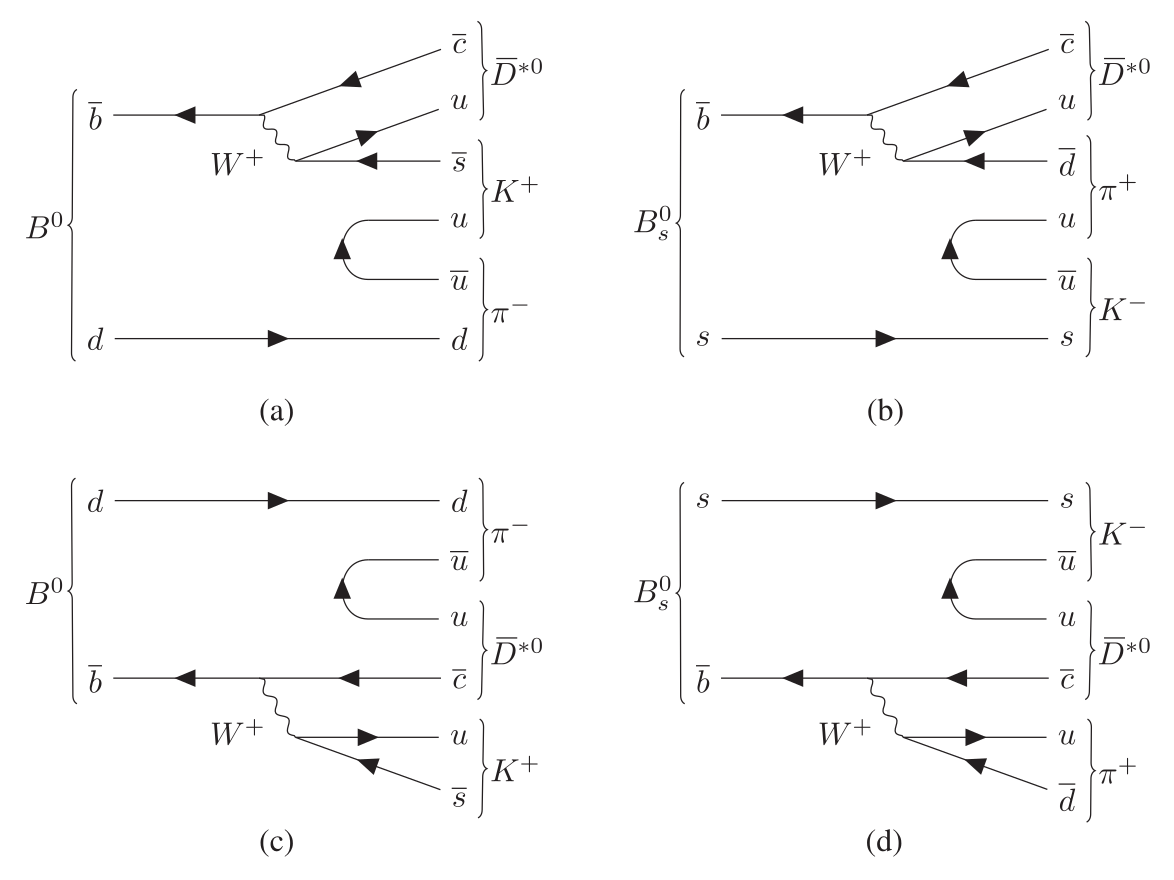
\includegraphics[width=.6\linewidth]{figures/conf/B2DKpi-fig001}
\end{frame}%}}}

\begin{frame}[label=B2DKpi-selection]%{{{
  \frametitle{$\Bz\to\Dstarzbar\Kp\pim$, $\Bsz\to\Dstarzbar\Km\pip$ event selection}

  \begin{itemize}
    \item Detector selection:
      $p_T$,
      distance from $pp$ interaction,
      secondary vertices.

    \item $\Dzbar\to\Kp\pim$ is used for $\Dzbar$.

    \item $\Dstarzbar\to\Dzbar\gamma$, $\Dzbar\piz$ are used for $\Dstarzbar$.

    \item $\Bz\to\Dstarzbar\pip\pim$ is used as normalization.

    \item A neural network is used to improve signal quality.
  \end{itemize}

  \centering
  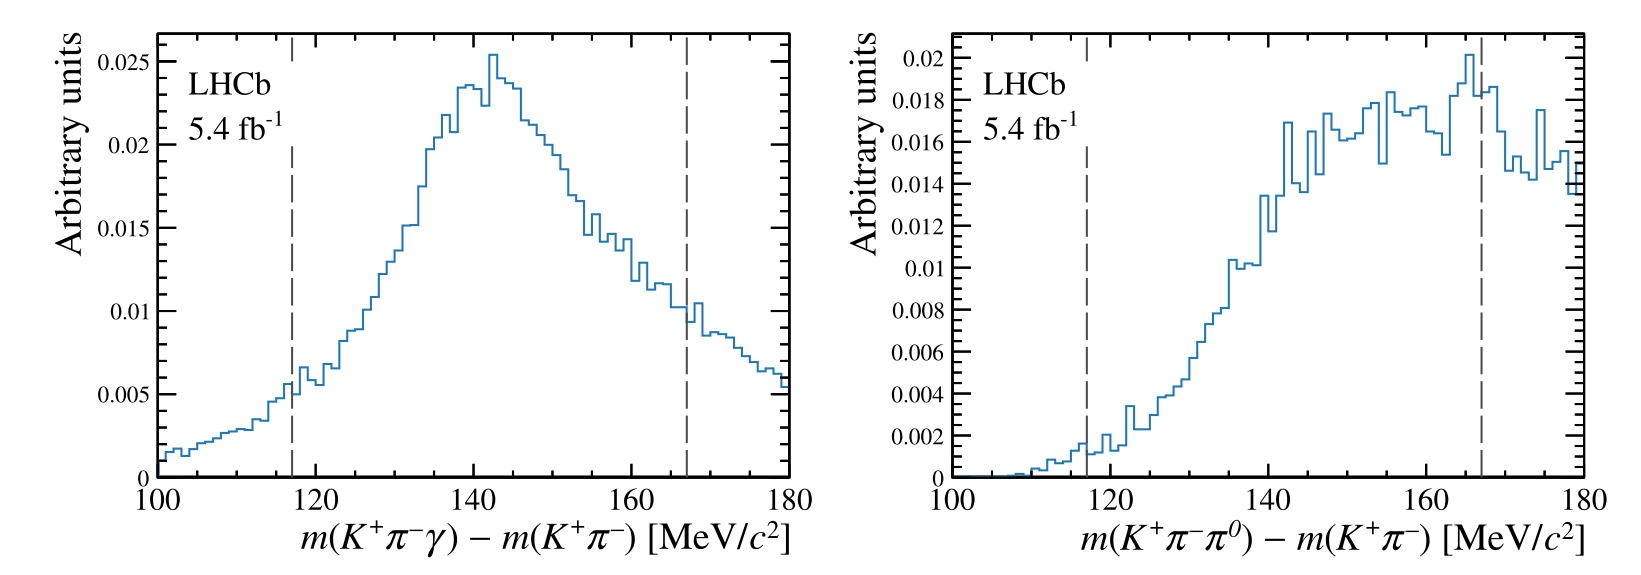
\includegraphics[width=.7\linewidth]{figures/conf/B2DKpi-fig002-pointless}
\end{frame}%}}}

\begin{frame}[label=B2DKpi-fit-top]%{{{
  %\frametitle{$\Bz\to\Dstarzbar\Kp\pim$, $\Bsz\to\Dstarzbar\Km\pip$,
  %$\Bsz\to\Dstarzbar\pip\pim$ models and fits}
  \frametitle{$\Bz\to\Dstarzbar\Kp\pim$ model and fit: components}
  \centering
  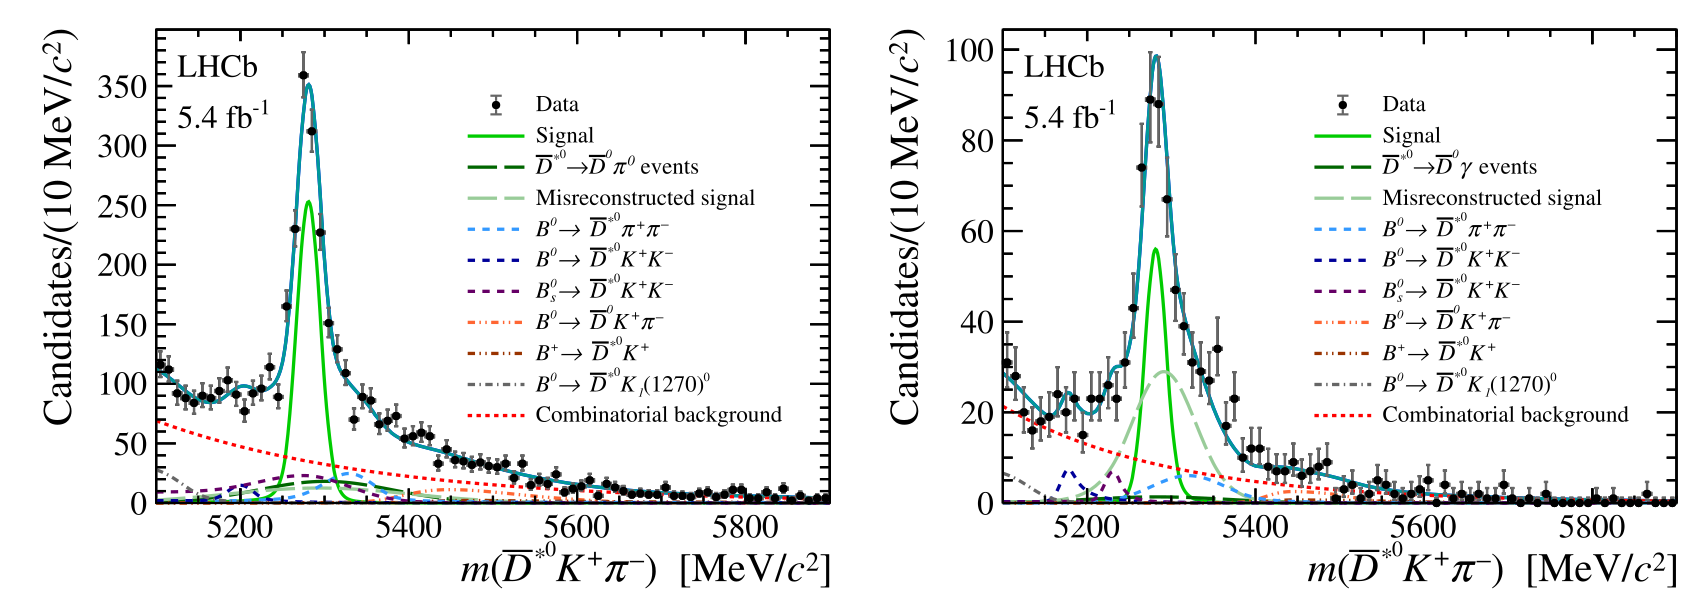
\includegraphics[width=.9\textwidth]{figures/conf/B2DKpi-fig003-top}

  \vfill
  Too many components: a simultaneous fit is required for stability $\to$
\end{frame}%}}}

\begin{frame}[label=B2DKpi-fit-mid-bot]%{{{
  \frametitle{$\Bsz\to\Dstarzbar\Km\pip$, $\Bz\to\Dstarzbar\pip\pim$ models and fits}
  \centering
  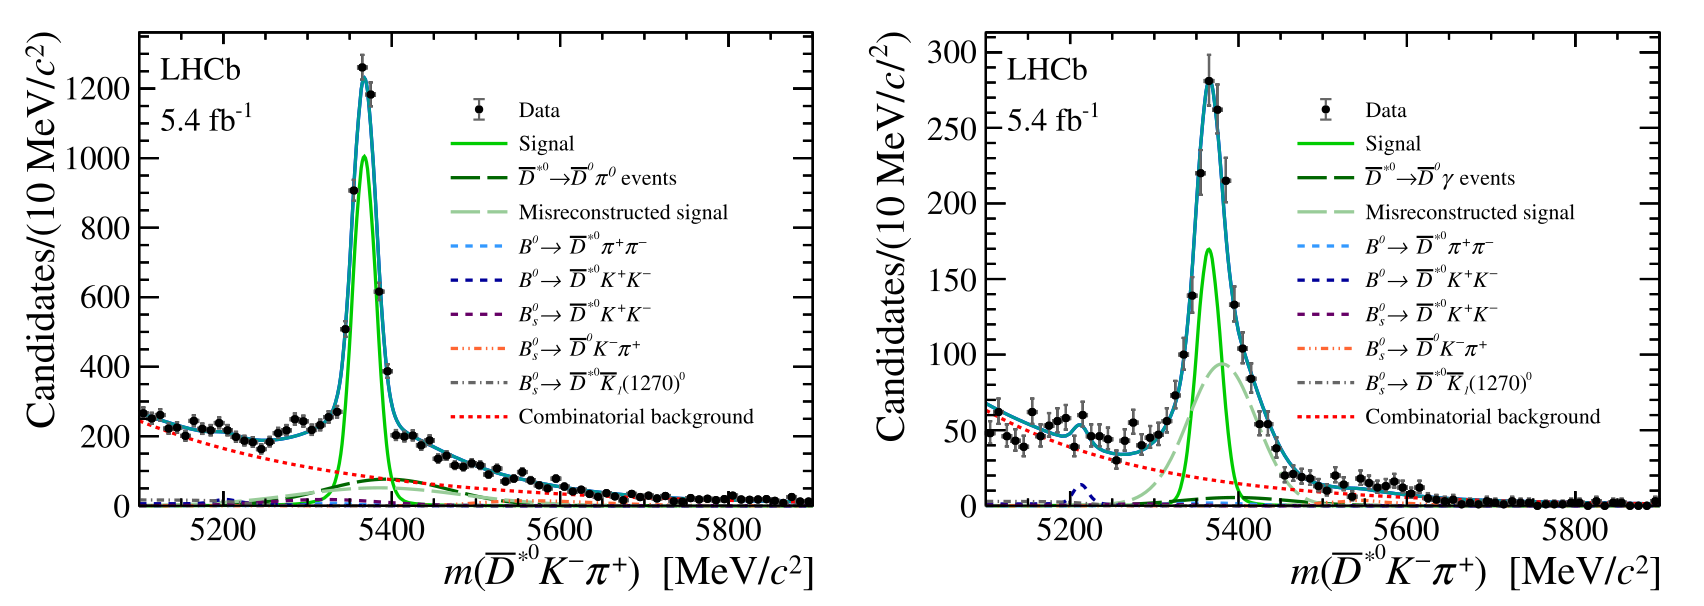
\includegraphics[width=.65\textwidth]{figures/conf/B2DKpi-fig003-mid}
  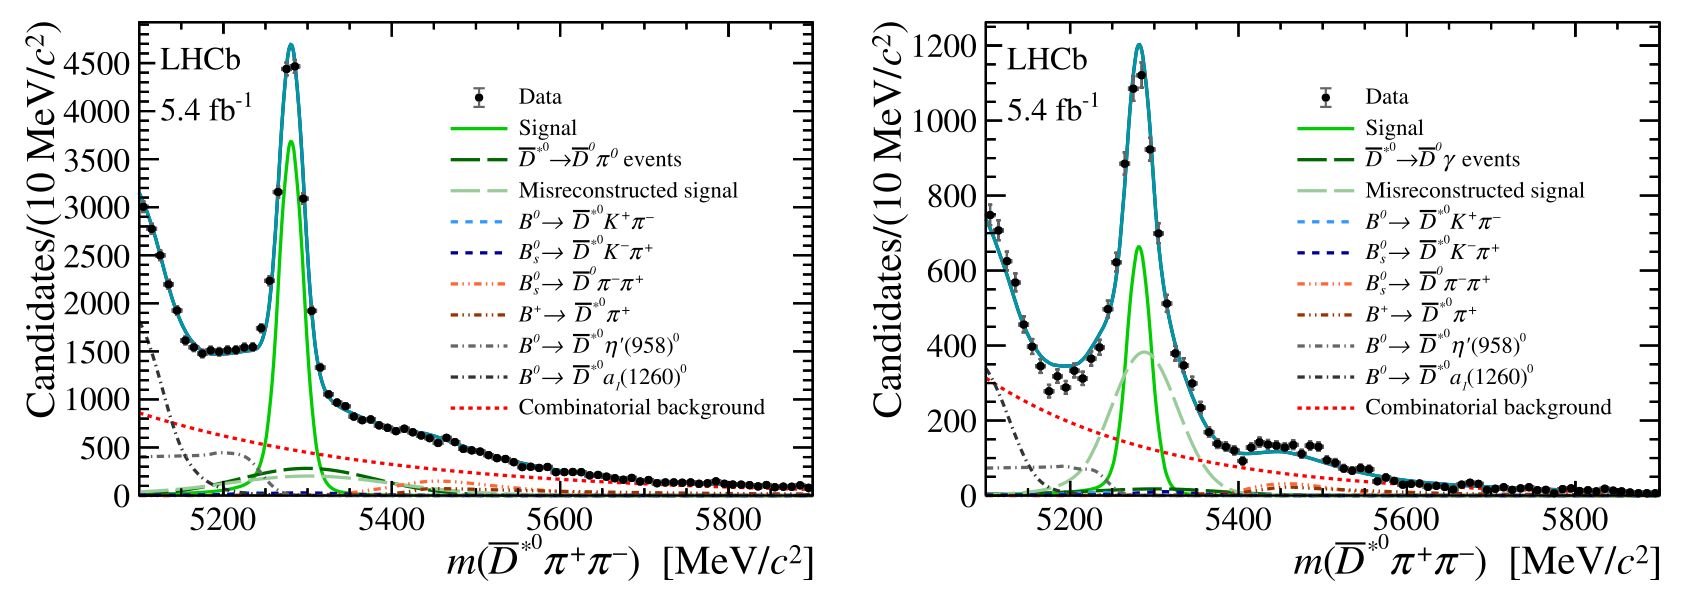
\includegraphics[width=.65\textwidth]{figures/conf/B2DKpi-fig003-bot}
\end{frame}%}}}

\begin{frame}[label=B2DKpi-eff]%{{{
  \frametitle{$\Bz\to\Dstarzbar\Kp\pim$, $\Bsz\to\Dstarzbar\Km\pip$,
  $\Bz\to\Dstarzbar\pip\pim$ efficiencies}

  Efficiencies are calculated across the whole phase space for each decay mode.

  The observed structures in efficiency-corrected plots support the approach.

  \vfill \centering
  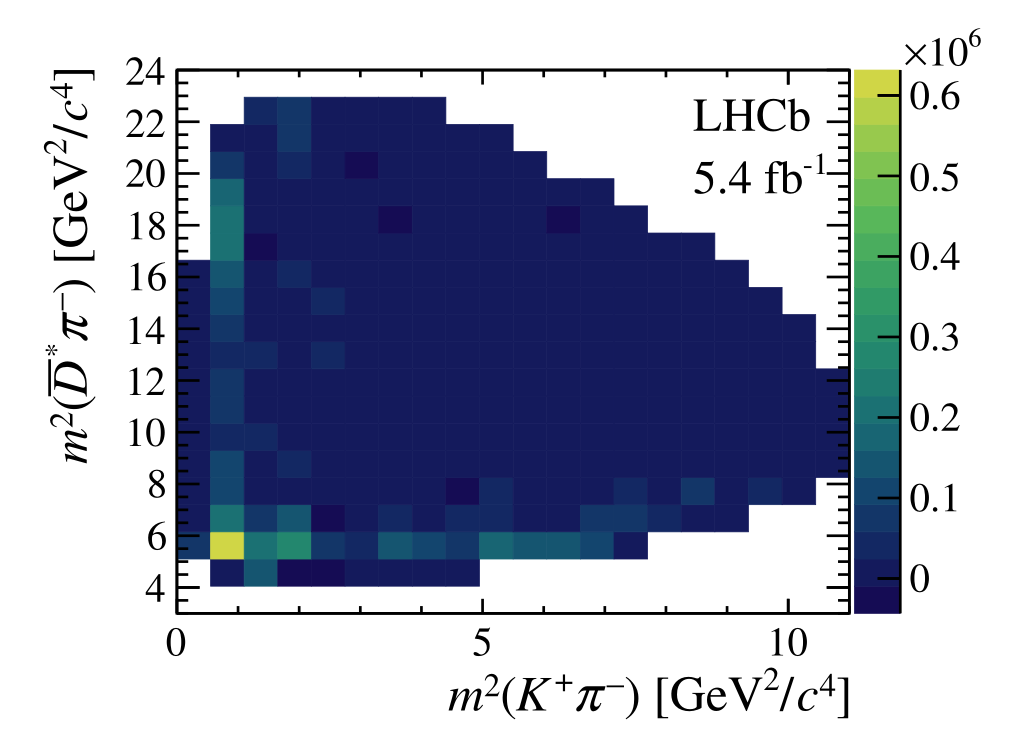
\includegraphics[width=.32\linewidth]{figures/conf/B2DKpi-fig006-top}
  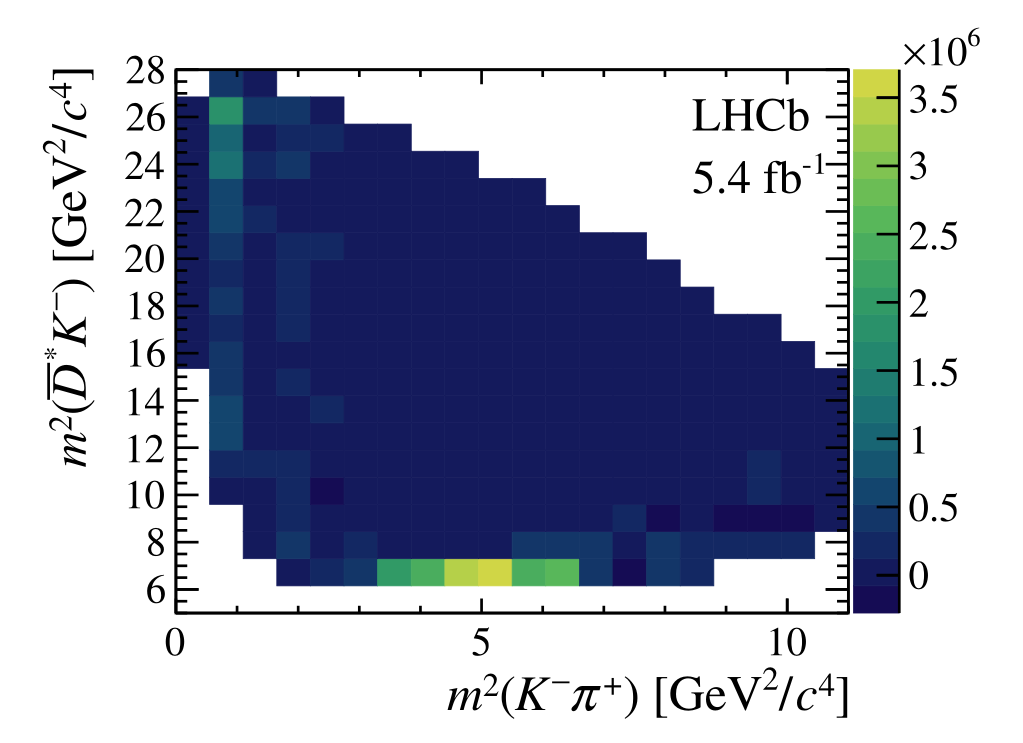
\includegraphics[width=.32\linewidth]{figures/conf/B2DKpi-fig006-mid}
  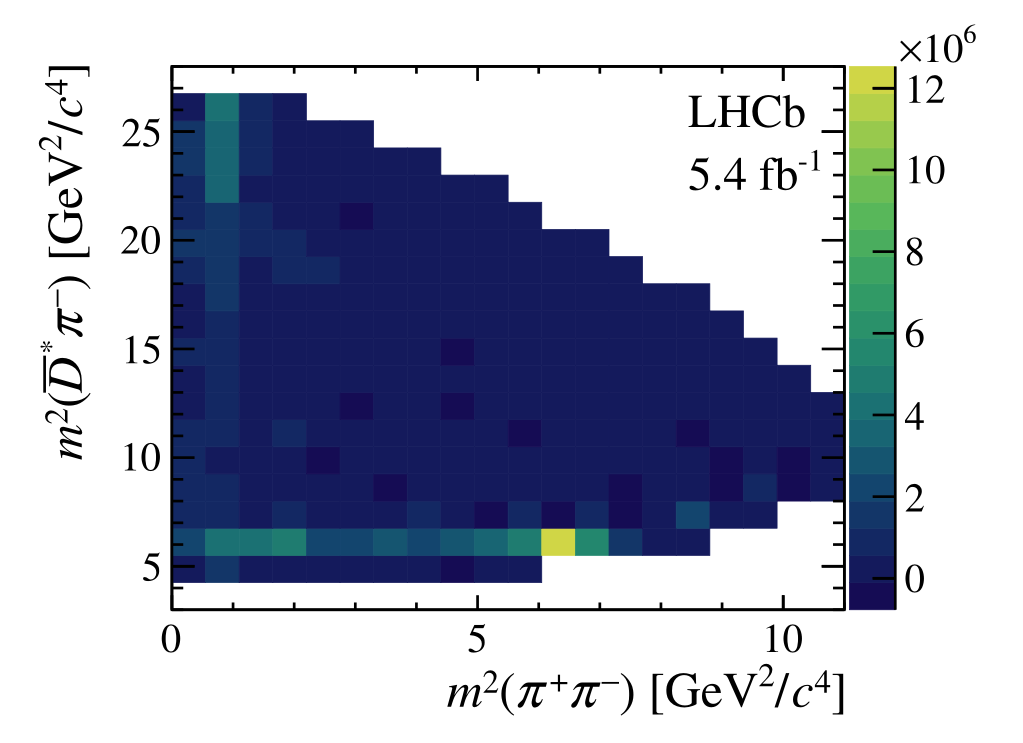
\includegraphics[width=.32\linewidth]{figures/conf/B2DKpi-fig006-bot}
\end{frame}%}}}

\begin{frame}[label=B2DKpi-syst]%{{{
  \frametitle{$\Bz\to\Dstarzbar\Kp\pim$, $\Bsz\to\Dstarzbar\Km\pip$,
  $\Bz\to\Dstarzbar\pip\pim$ systematics}

  \centering
  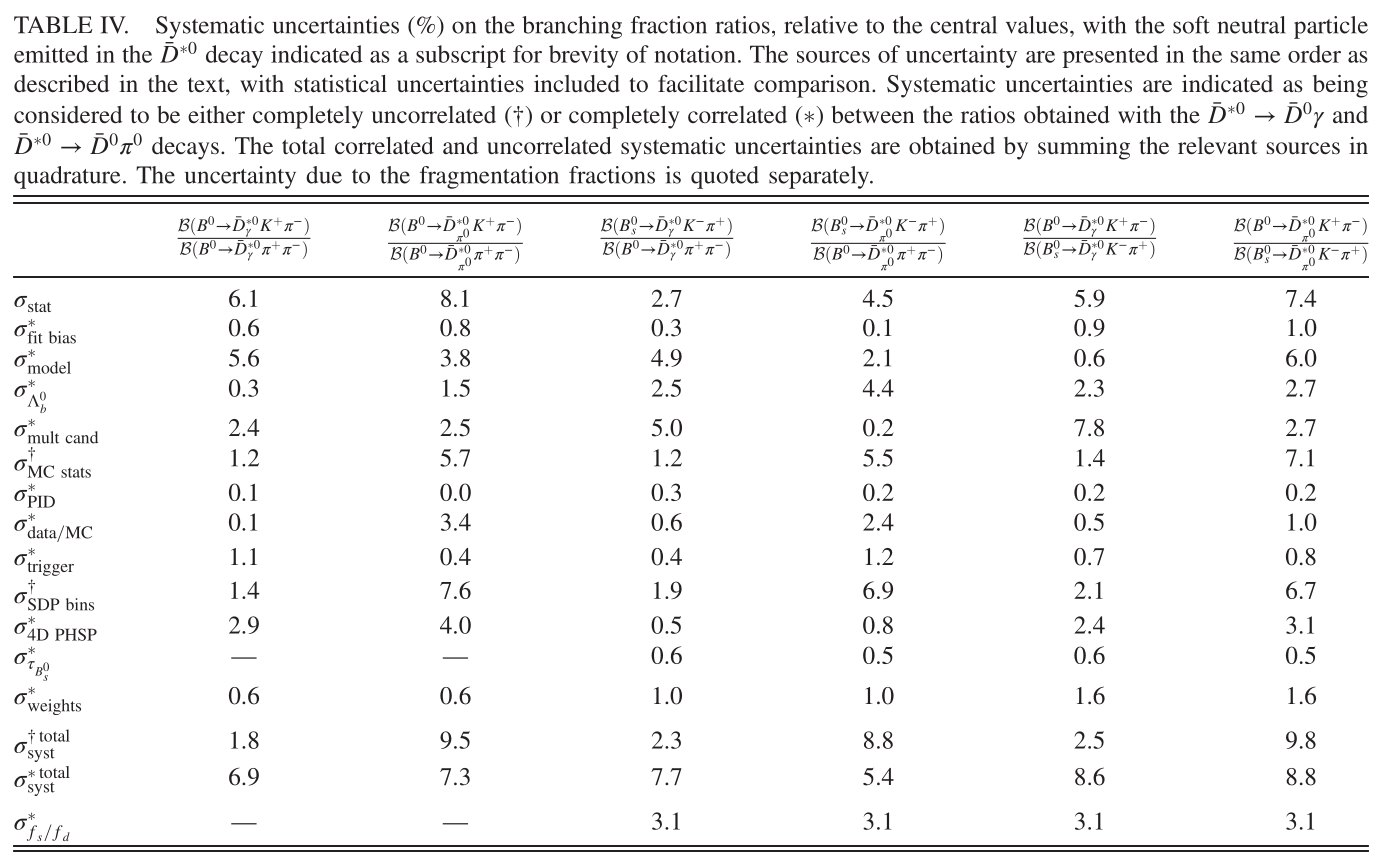
\includegraphics[width=.7\linewidth]{figures/conf/B2DKpi-tab005}
\end{frame}%}}}

\begin{frame}[label=B2DKpi-results]%{{{
  \frametitle{$\Bz\to\Dstarzbar\Kp\pim$, $\Bsz\to\Dstarzbar\Km\pip$,
  $\Bz\to\Dstarzbar\pip\pim$ results}

  \centering
  \parbox{.55\linewidth}{
    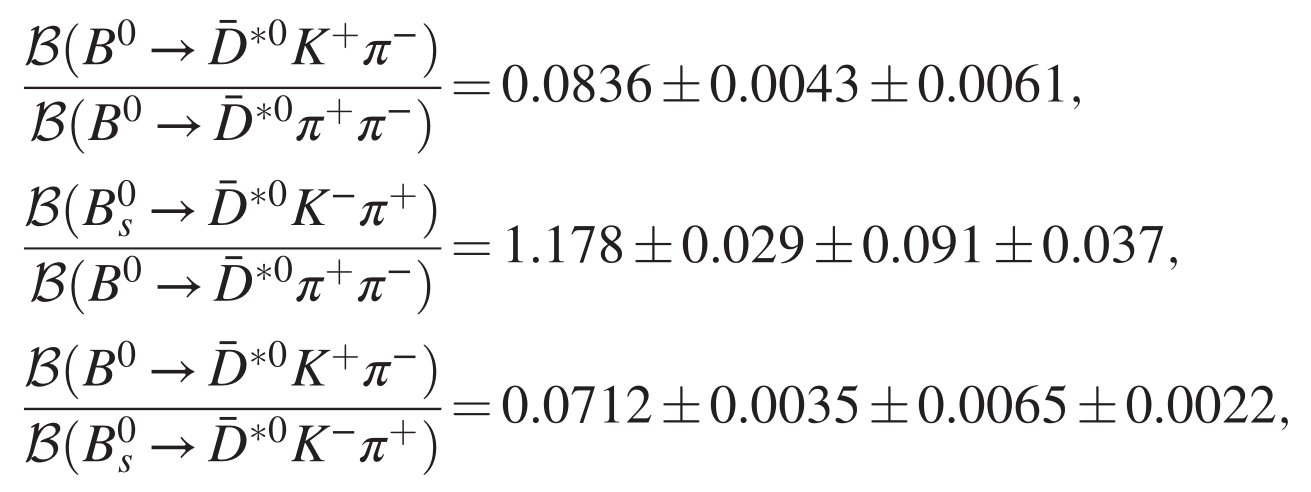
\includegraphics[width=\linewidth]{figures/conf/B2DKpi-txt001-results}
  } \hfill \vfill \parbox{.99\linewidth}{
    \begin{itemize}
      \item The results are averaged considering the correlation
        between $\Dstarzbar$ modes.
      \item The significances are well over $5\sigma$.
      \item Two new decays are observed and measured.
      \item The results and the Dalitz plots are useful to suppress 
        systematics in future CKM $\gamma$ measurements.
    \end{itemize}
  }
\end{frame}%}}}

\begin{frame}[label=Lb2Dppipi-intro]%{{{
  \frametitle{$\Lb\to\Dp p\pim\pim$ quark diagram}

  \begin{itemize}
    \item The decays $\Lb\to\Dp p\pim\pim$ and $\Lb\to\Dstarp p\pim\pim$
      are nonleptonic and multihadron.
    \item Different final state hadrons carry the $c$-quark
      and the baryon number.
    \item The decays sensitive to hadronization
      as well as hadron spectroscopy.
  \end{itemize}

  \vfill \centering
  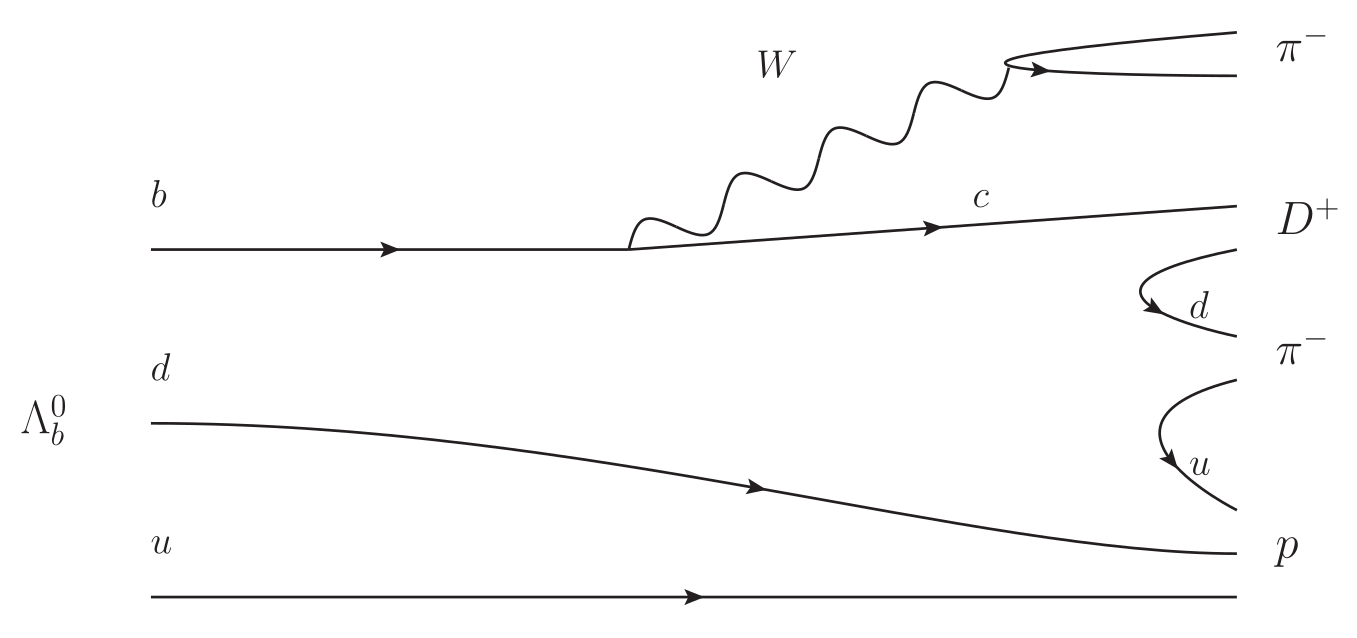
\includegraphics[width=.6\linewidth]{figures/conf/Lb2Dppipi-fig000}
\end{frame}%}}}

\begin{frame}[label=Lb2Dppipi-selection]%{{{
  \frametitle{$\Lb\to\Dp p\pim\pim$, $\Lb\to\Dstarp p\pim\pim$,
  $\Lb\to\Lc\pip\pim\pim$ event selection}

  \begin{itemize}
    \item Detector selection:
      $p_T$,
      distance from $pp$ interaction,
      secondary vertices.

    \item $\Dp\to\Km\pip\pip$ is used for $\Dp$.

    \item $\Dstarp\to\Dp\piz$, $\Dp\gamma$ are used for $\Dstarp$.

    \item $\Lc\to p\Km\pip$ is used for $\Lc$.

    \item Kinematic cuts suppress the background.

    \item Normalization $\Lb\to\Lc\pip\pim\pim$ events are simulated 
      considering their resonance structure.
  \end{itemize}
\end{frame}%}}}

\begin{frame}[label=Lb2Dppipi-fit]%{{{
  \frametitle{$\Lb\to\Dp p\pim\pim$, $\Lb\to\Dstarp p\pim\pim$,
  $\Lb\to\Lc\pip\pim\pim$ models and fits}

  \centering
  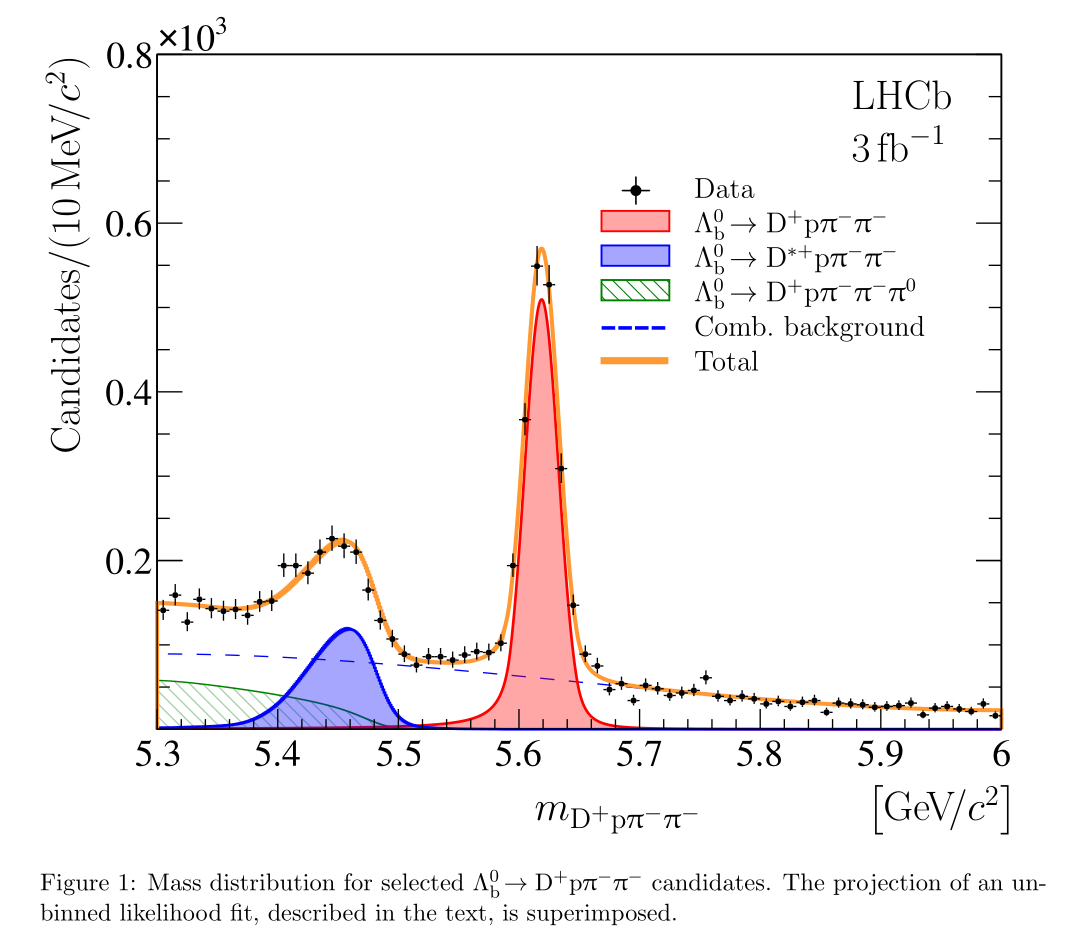
\includegraphics[width=.49\linewidth]{figures/conf/Lb2Dppipi-fig001}
  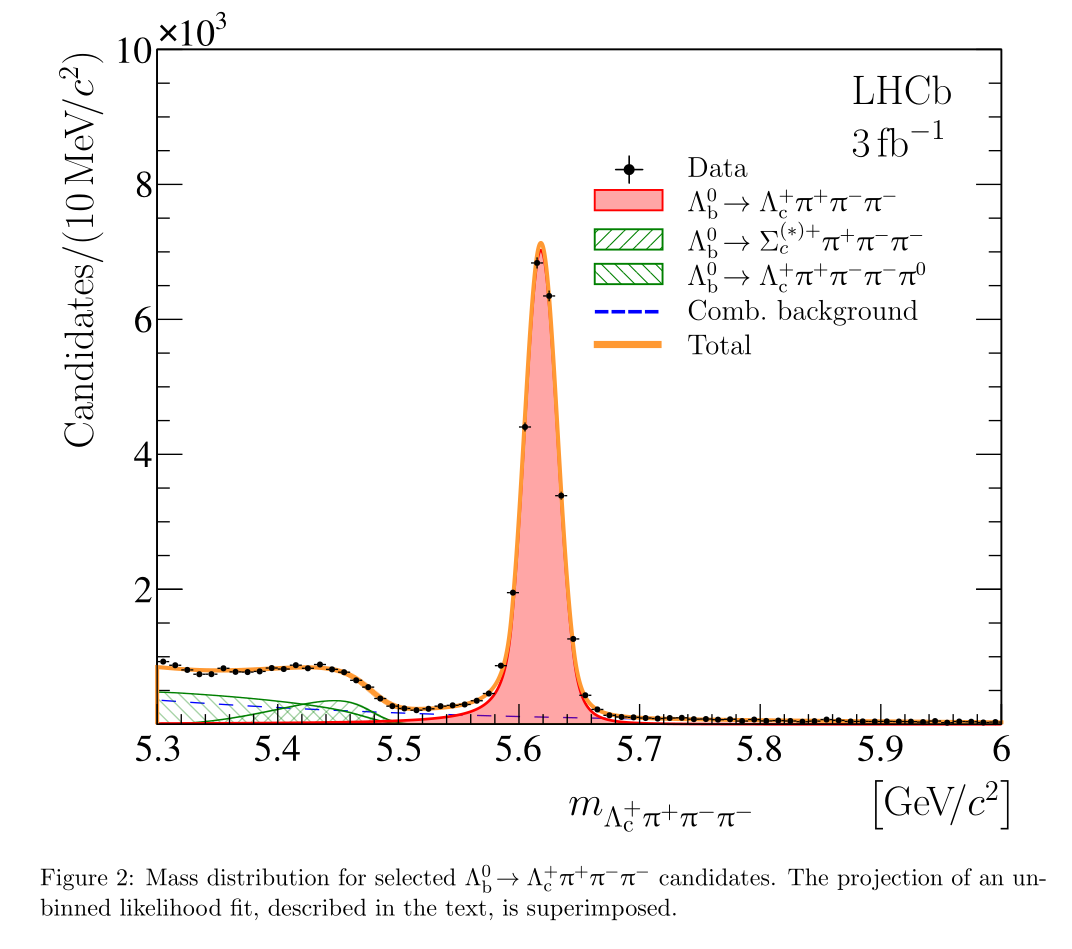
\includegraphics[width=.49\linewidth]{figures/conf/Lb2Dppipi-fig002}
\end{frame}%}}}

\begin{frame}[label=Lb2Dppipi-fit-corr]%{{{
  \frametitle{$\Lb\to D^{(*)+} p \pim\pim$ cross section,
  double counting, $D_s$ contribution}

  \centering
  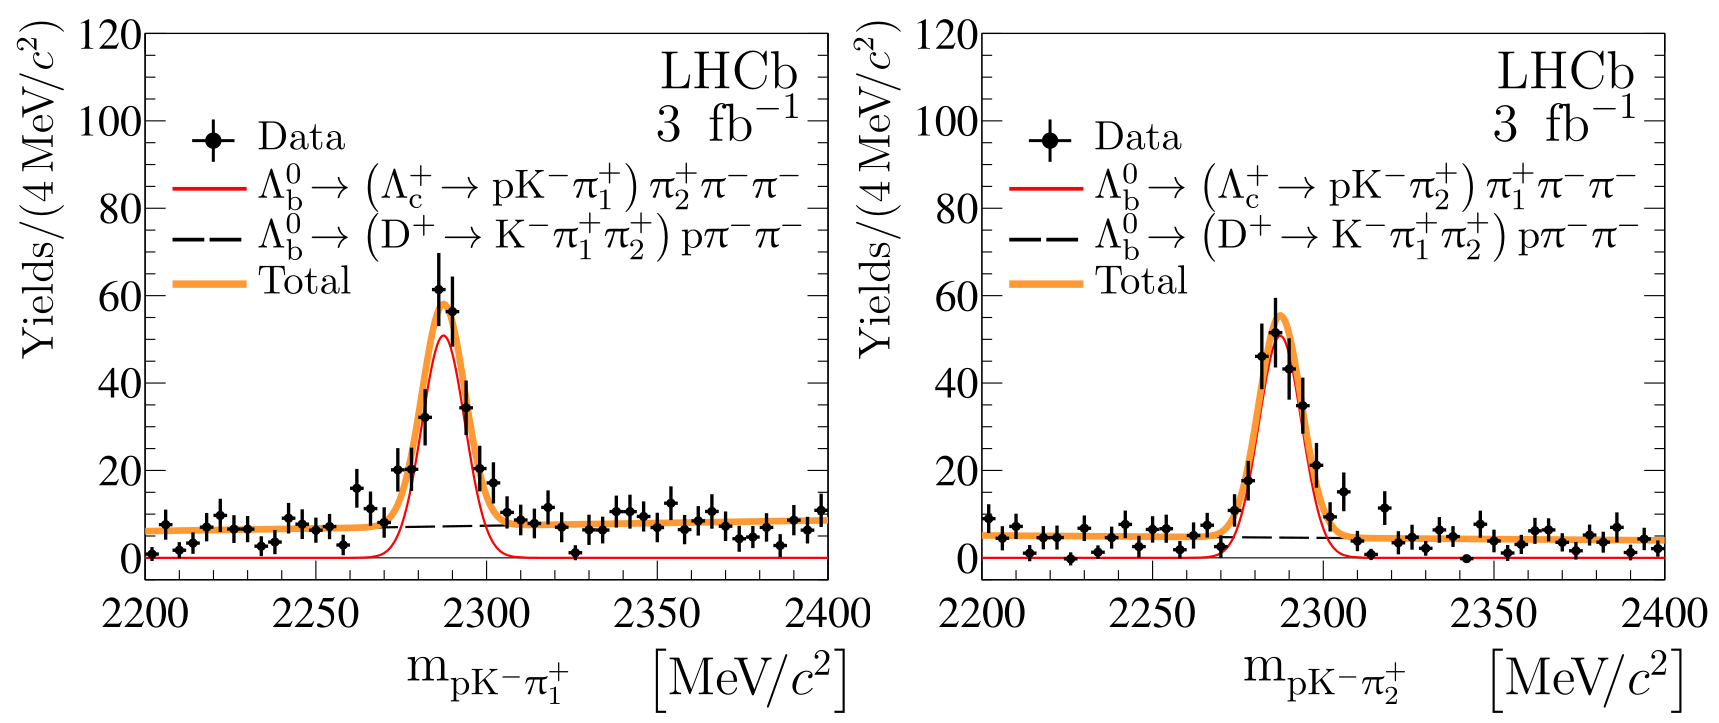
\includegraphics[width=.56\linewidth]{figures/conf/Lb2Dppipi-fig003}
  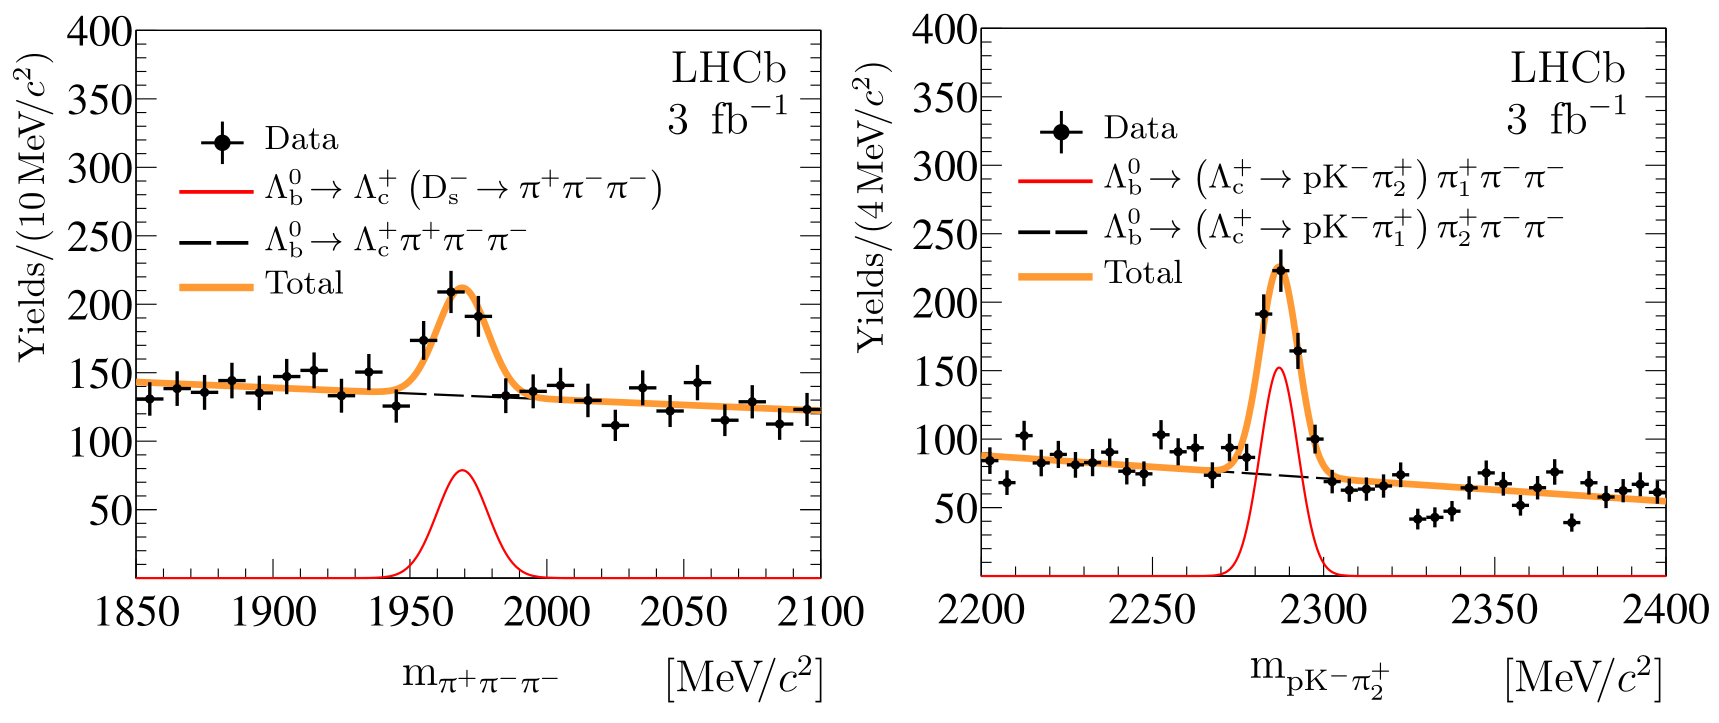
\includegraphics[width=.56\linewidth]{figures/conf/Lb2Dppipi-fig004}
\end{frame}%}}}

\begin{frame}[label=Lb2Dppipi-eff]%{{{
  \frametitle{$\Lb\to D^{(*)+} p \pim\pim$ efficiencies}

  \begin{itemize}
    \item Efficiencies are calculated based on simulation.
    \item The simulation is reweighted to better represent the data.
  \end{itemize}

  \centering
  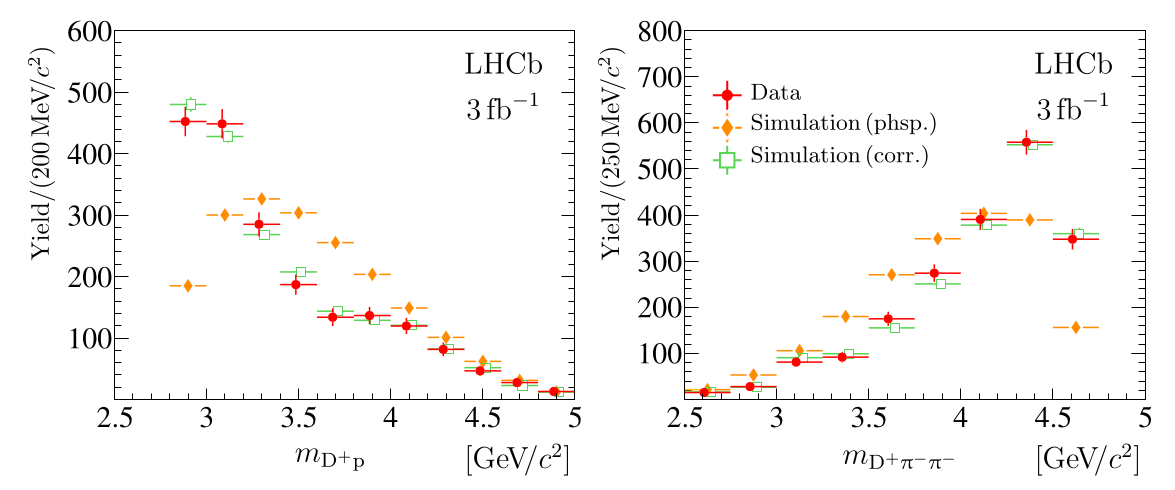
\includegraphics[width=.45\linewidth]{figures/conf/Lb2Dppipi-fig005-1}
  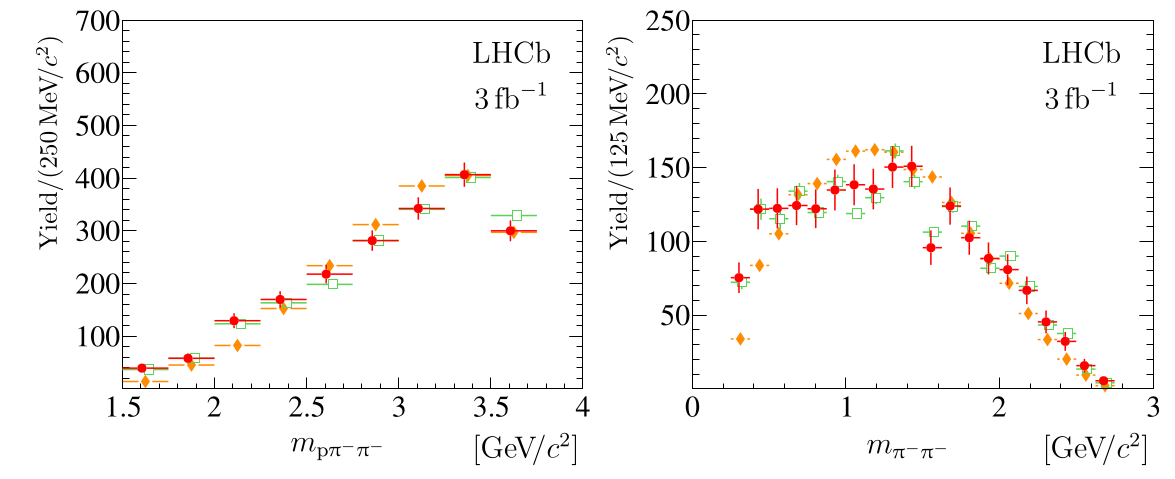
\includegraphics[width=.45\linewidth]{figures/conf/Lb2Dppipi-fig005-2}
  \includegraphics[width=.45\linewidth]{figures/conf/Lb2Dppipi-fig005-3}
  \includegraphics[width=.45\linewidth]{figures/conf/Lb2Dppipi-fig006-1}
\end{frame}%}}}

\begin{frame}[label=Lb2Dppipi-syst]%{{{
  \frametitle{$\Lb\to D^{(*)+} p \pim\pim$ systematics}

  \centering
  \includegraphics[width=.75\linewidth]{figures/conf/Lb2Dppipi-tab002}
\end{frame}%}}}

\begin{frame}[label=Lb2Dppipi-results]%{{{
  \frametitle{$\Lb\to D^{(*)+} p \pim\pim$ results}

  \centering
  $$\mathcal{R}_{\Dp} =
  \frac{\mathcal{B}\left(\Lb\to\Dp p\pim\pim\right)}
  {\mathcal{B}\left(\Lb\to\Lc\pip\pim\pim\right)}
  \times
  \frac{\mathcal{B}\left(\Dp\to\Km\pip\pip\right)}
  {\mathcal{B}\left(\Lc\to p\Km\pip\right)}
  = (5.35\pm0.21\pm0.16)\%$$

  $$\mathcal{R}_{\Dstarp} =
  \frac{\mathcal{B}\left(\Lb\to\Dstarp p\pim\pim\right)}
  {\mathcal{B}\left(\Lb\to\Dp p\pim\pim\right)}
  \times
  \mathcal{B}\left(\Dstarp\to\Dp\piz,\ \Dp\gamma\right)
  = (61.3\pm4.3\pm4.0)\%$$

  \begin{itemize}
    \item The ratio of $\Dstarp$ to $\Dp$ mesons derived from 
      $\mathcal{R}_\Dstarp$ is similar to the one from $ee$ collisions.
      The hadronization is similar.
    \item The $\Lb\to\Sigma_c^{(*)+}\pip\pim\pim$ is not measured, but 
      heavily suppressed, just like in $ee$ collisions.
    \item First observation and measurement of both decays.
    \item The two decays, as well as the normalization channel, have 
      a rich resonance structure.
  \end{itemize}
\end{frame}%}}}

\end{document}
